\documentclass[a4paper]{report}

\usepackage{../mathstemplate}

\date{IV семестр, весна 2024 г.}
\title{Алгебра. Неофициальный конспект}
\author{Лектор: Алексей Владимирович Степанов\\ Конспектировал Леонид Данилевич}

\begin{document}
    \shorthandoff{"}
    \maketitle
    \tableofcontents
    \newpage
    \setcounter{lection}{0}


    \chapter{Гомологическая алгебра}
    \newlection{12 февраля 2024 г.}


    \section{Абелевы категории}
    Напомним некоторые определения из предыдущей лекции.
    \definition[Предаддитивная категория $\cat{A}$]{
        $\forall A, B \in \cat{A}: \Mor_{\cat{A}}(A, B)$ образует абелеву группу, и везде, где определена, выполнена дистрибутивность: \[\alpha(\beta+\gamma) = \alpha\beta + \alpha\gamma \qquad (\beta + \gamma)\alpha = \beta\alpha + \gamma\alpha\]
    }
    \definition[Бипроизведение]{ Такая диаграмма, что
    % https://q.uiver.app/#q=WzAsMyxbMSwwLCJDIl0sWzAsMCwiQSJdLFsyLDAsIkIiXSxbMSwwLCJcXGlvdGFfMSIsMix7Im9mZnNldCI6MX1dLFswLDEsIlxccGlfMSIsMix7Im9mZnNldCI6MX1dLFswLDIsIlxccGlfMiIsMCx7Im9mZnNldCI6LTF9XSxbMiwwLCJcXGlvdGFfMiIsMCx7Im9mZnNldCI6LTF9XV0=
        \[\begin{tikzcd}[ampersand replacement=\&]
              A \& C \& B
              \arrow["{\iota_1}"', shift right, from=1-1, to=1-2]
              \arrow["{\pi_1}"', shift right, from=1-2, to=1-1]
              \arrow["{\pi_2}", shift left, from=1-2, to=1-3]
              \arrow["{\iota_2}", shift left, from=1-3, to=1-2]
        \end{tikzcd}\]
        \numbers{
            \item $\pi_1\iota_1 = \id_A$.
            \item $\pi_2\iota_2 = \id_B$.
            \item $ \iota_2 \pi_2+ \iota_1\pi_1  = \id_C$.
            \item $\pi_2\iota_1 = 0$.
            \item $\pi_1\iota_2 = 0$.
        }
    }
    \definition[Аддитивная категория]{
        Предаддитивная категория с финальным объектом и произведениями (любых двух объектов).
    }
    Эквивалентно, существуют инициальный объект и копроизведения, эквивалентно существуют нулевой объект и бипроизведения.
    \definition[Предабелева категория]{
        Аддитивная категория, в которой у всех морфизмов есть ядро и коядро.
    }
    \definition[(Ко)нормальный мономорфизм (эпиморфизм)]{
        Он является (ко)эквалайзером (какой-то, неважно какой, пары стрелок).
    }
    \definition[Абелева категория]{
        Предабелева категория, в которой все мономорфизмы нормальны.
    }
    Пусть $\cat C$ --- категория.
    Вспомним про категорию стрелок $\cat{Arr}\cat{C}$, в которой объекты --- стрелки из $\Mor(\cat C)$, множество морфизмов между $\phi, \psi$ --- это\[\Mor_{\cat{Arr}_{\cat{C}}}(\phi, \psi) = \defset{(\alpha, \beta)}{\alpha: \source(\phi) \map \source(\psi), \beta: \target(\phi) \map \target(\psi), \beta \phi = \psi \alpha}\]
    % https://q.uiver.app/#q=WzAsNCxbMCwwLCJcXGJ1bGxldCJdLFsxLDAsIlxcYnVsbGV0Il0sWzAsMSwiXFxidWxsZXQiXSxbMSwxLCJcXGJ1bGxldCJdLFswLDEsIlxccGhpIl0sWzIsMywiXFxwc2kiXSxbMCwyLCJcXGFscGhhIl0sWzEsMywiXFxiZXRhIl1d
    \[\begin{tikzcd}[ampersand replacement=\&]
          \bullet \& \bullet \\
          \bullet \& \bullet
          \arrow["\phi", from=1-1, to=1-2]
          \arrow["\psi", from=2-1, to=2-2]
          \arrow["\alpha", from=1-1, to=2-1]
          \arrow["\beta", from=1-2, to=2-2]
    \end{tikzcd}\]
    Далее будем обозначать за $\ker f$ ядро стрелки, как уравнитель стрелки и нуля, а за $\Ker f \coloneqq \source(\ker f)$ --- объект (в конкретных категориях типа $\modR{R}$ это докатегорное понятие ядра --- подмодуль без стрелки-вложения).
    \lemma{\label{ker-is-functor}
        $\ker, \coker$ --- функторы $\cat{Arr} \cat A \map \cat{Arr} \cat A$.
        \provehere{
            Достаточно доказать для ядер, для коядер двойственно.

            Определим действие $\ker$ на морфизмах:
        % https://q.uiver.app/#q=WzAsNixbMSwwLCJBIl0sWzEsMSwiQSciXSxbMiwwLCJCIl0sWzIsMSwiQiciXSxbMCwwLCJcXEtlciBmIl0sWzAsMSwiXFxLZXIgZiciXSxbMCwyLCJmIl0sWzEsMywiZiciXSxbMCwxLCJcXGFscGhhIl0sWzIsMywiXFxiZXRhIl0sWzQsMCwiXFxrZXIgZiJdLFs1LDEsIlxca2VyIGYnIl0sWzQsNSwiXFxleGlzdHMhXFxwaGkiLDAseyJsYWJlbF9wb3NpdGlvbiI6NDAsInN0eWxlIjp7ImJvZHkiOnsibmFtZSI6ImRhc2hlZCJ9fX1dXQ==
            \[\begin{tikzcd}[ampersand replacement=\&]
            {\Ker f}
                  \& A \& B \\
                  {\Ker f'} \& {A'} \& {B'}
                  \arrow["f", from=1-2, to=1-3]
                  \arrow["{f'}", from=2-2, to=2-3]
                  \arrow["\alpha", from=1-2, to=2-2]
                  \arrow["\beta", from=1-3, to=2-3]
                  \arrow["{\ker f}", from=1-1, to=1-2]
                  \arrow["{\ker f'}", from=2-1, to=2-2]
                  \arrow["{\exists!\phi}"{pos=0.4}, dashed, from=1-1, to=2-1]
            \end{tikzcd}\]
            $f \cdot \ker f = 0 \then \beta \cdot f \cdot \ker f = 0 \then f' \cdot \alpha \cdot \ker f = 0$, откуда по универсальному свойству ядра $\exists !\phi: \ker f' \cdot \phi = \alpha \cdot \ker f$.

            Положим $\ker(\alpha, \beta) = (\phi, \alpha)$.
            Далее несложно проверить, что данное определение сохраняет композицию и $\id$.
        }
    }
    \definition[Точный функтор]{Функтор, сохраняющий ядра и коядра.}
    \intfact[Теорема Фрейда --- Митчелла (Freyd --- Mitchell)] {\label{mitchell}
    Для любой малой абелевой категории $\cat{A}$: $\exists R \in \cat{Ring}$ (необязательно коммутативное кольцо с единицей) и строгий, полный, точный функтор $\cat{A} \map \modR{R}$.
    }
    \proposal{
        Для всякого морфизма $f: A \map B$ найдётся пунктирная стрелка, делающая диаграмму коммутативной.
% https://q.uiver.app/#q=WzAsNixbMCwwLCJcXEtlciBmIl0sWzEsMCwiQSJdLFsyLDAsIkIiXSxbMywwLCJcXENvS2VyIGYiXSxbMSwxLCJcXENvS2VyIFxca2VyIGYiXSxbMiwxLCJcXEtlciBcXGNva2VyIGYiXSxbMSwyLCJmIl0sWzAsMSwiXFxrZXIgZiJdLFsyLDMsIlxcY29rZXIgZiJdLFsxLDQsIlxcY29rZXJcXGtlciBmIiwyXSxbNSwyLCJcXGtlciBcXGNva2VyIGYiLDJdLFs0LDUsIlxcZXhpc3RzISIsMCx7InN0eWxlIjp7ImJvZHkiOnsibmFtZSI6ImRhc2hlZCJ9fX1dXQ==
        \[\begin{tikzcd}[ampersand replacement=\&]
        {\Ker f}
              \& A \& B \& {\CoKer f} \\
              \& {\CoKer \ker f} \& {\Ker \coker f}
              \arrow["f", from=1-2, to=1-3]
              \arrow["{\ker f}", from=1-1, to=1-2]
              \arrow["{\coker f}", from=1-3, to=1-4]
              \arrow["{\coker\ker f}"', from=1-2, to=2-2]
              \arrow["{\ker \coker f}"', from=2-3, to=1-3]
              \arrow["{\exists!}", dashed, from=2-2, to=2-3]
        \end{tikzcd}\]
        Более того, в абелевой категории эта стрелка --- изоморфизм.
        \provehere{
            Следует из эпи-моно разложения, доказанного на прошлой лекции, или из теоремы Митчелла.

            Само построение пунктирной стрелки получается из универсальных свойств, а доказательство того, что это --- изо --- непростое.
        }
    }
    \lemma{\label{when-ab} Пусть $\cat C$ --- полная подкатегория в абелевой категории $\cat A$. Следующие условия равносильны
    \bullets{
        \item $\cat C$ является абелевой.
        \item \bullets{
            \item $0_{\cat A} \in \cat C$, здесь, как обычно, $0_{\cat A}$ --- нулевой объект категории $\cat A$.
            \item $\cat C$ содержит бипроизведение любых двух своих объектов.
            \item Ядра и коядра (взятые в $\cat A$) любых морфизмов из $\cat C$ лежат в $\cat C$.
        }
    }
    \provewthen{
        Очевидно.
    }{
        Чуть сложнее, доказывать не будем (и использовать тоже).
    }
    }


    \section{Компл$\acute{\text{е}}$ксы}
    Если противное не оговорено, то всё происходит в абелевой категории $\cat A$, большими буквами обозначены объекты данной категории, маленькими --- морфизмы.
    \definition[Компл$\acute{\text{е}}$кс]{
        Такая диаграмма, что $\forall k \in \Z: d_k \cdot d_{k+1} = 0$.
        % https://q.uiver.app/#q=WzAsNSxbMSwwLCJDX3tuKzF9Il0sWzIsMCwiQ19uIl0sWzMsMCwiQ197bi0xfSJdLFswLDAsIlxcY2RvdHMiXSxbNCwwLCJcXGNkb3RzIl0sWzMsMCwiZF97bisxfSJdLFswLDEsImRfbiJdLFsxLDIsImRfe24tMX0iXSxbMiw0LCJkX3tuLTJ9Il1d
        \[\begin{tikzcd}[ampersand replacement=\&]
              \cdots \& {C_{n+1}} \& {C_n} \& {C_{n-1}} \& \cdots
              \arrow["{d_{n+1}}", from=1-1, to=1-2]
              \arrow["{d_n}", from=1-2, to=1-3]
              \arrow["{d_{n-1}}", from=1-3, to=1-4]
              \arrow["{d_{n-2}}", from=1-4, to=1-5]
        \end{tikzcd}\]
    }
    Альтернативно, комплекс можно рассматривать, как функтор из категории $(\Z, \ge)$ (полученной из частично упорядоченного множества) в $\cat A$ (при котором образ композиции любых двух нетождественных морфизмов нулевой).
    Таким образом, комплексы --- полная подкатегория в категории этих функторов.

    Ещё один, следующий, взгляд на комплексы работает только для конкретной категории, уже вложенной в $R$-модули.
    \definition[Градуированный объект]{
        $C_{\bullet} = \bigoplus\limits_{n \in \Z}C_n$ с морфизмом $d: C_\bullet \map C_\bullet$, таким, что $d(C_n) \subset C_{n+p}$ для некоторой фиксированной \emph{степени объекта} $p$ (чаще всего она равна $\pm1$).
    }
    \definition[Дифференциальный модуль]{
        Градуированный объект $(C_\bullet, d)$ со свойством $d^2 = 0$.
    }
    \definition[Комплекс]{ Дифференциальный модуль степени $-1$. }
    При развороте стрелок получается дифференциальный модуль степени $+1$, также известный, как \emph{кокомплекс}:
    % https://q.uiver.app/#q=WzAsNSxbMCwwLCJcXGNkb3RzIl0sWzEsMCwiQ157bisxfSJdLFsyLDAsIkNee259Il0sWzMsMCwiQ157bi0xfSJdLFs0LDAsIlxcY2RvdHMiXSxbMSwwLCJkXntuKzJ9IiwyXSxbMiwxLCJkXntuKzF9IiwyXSxbMywyLCJkXm4iLDJdLFs0LDMsImRee24tMX0iLDJdXQ==
    \[\begin{tikzcd}[ampersand replacement=\&]
          \cdots \& {C^{n+1}} \& {C^{n}} \& {C^{n-1}} \& \cdots
          \arrow["{d^{n+2}}"', from=1-2, to=1-1]
          \arrow["{d^{n+1}}"', from=1-3, to=1-2]
          \arrow["{d^n}"', from=1-4, to=1-3]
          \arrow["{d^{n-1}}"', from=1-5, to=1-4]
    \end{tikzcd}\]
    \precaution{
        У кокомплекса несколько другая нумерация стрелок, но мы их практически не будем использовать.
    }
    \definition[Сдвиг комплекса $(C_\bullet, d)$ на $p \in \Z$]{
        Комплекс $(C[p]_\bullet, d[p])$, где $C[p]_n = C_{n+p}$ и $d[p]_n = d_{n+p}$.
    }
    Иногда при сдвиге комплекса определяют $d[p]_n = (-1)^p d_{n+p}$, но мы так делать не будем.
    \newlection{19 февраля 2024 г.}
    \definition[Морфизм дифференциальных модулей $\bigoplus A_n \map \bigoplus B_n$]{
        Такое $f: \bigoplus A_n \map \bigoplus B_n$, что $f(A_n) \subset B_n$, и диаграммы коммутативны:
        % https://q.uiver.app/#q=WzAsNCxbMCwwLCJBX3tuKzF9Il0sWzEsMCwiQV9uIl0sWzAsMSwiQl97bisxfSJdLFsxLDEsIkJfbiJdLFswLDEsImRfbl5BIl0sWzIsMywiZF9uXkIiXSxbMCwyLCJmIl0sWzEsMywiZiJdXQ==
        \[\begin{tikzcd}[ampersand replacement=\&]
        {A_{n+1}}
              \& {A_n} \\
              {B_{n+1}} \& {B_n}
              \arrow["{d_n^A}", from=1-1, to=1-2]
              \arrow["{d_n^B}", from=2-1, to=2-2]
              \arrow["f", from=1-1, to=2-1]
              \arrow["f", from=1-2, to=2-2]
        \end{tikzcd}\]
        На языке абелевых категорий, надо рассматривать не одно отображение $f$, так как отношение $f(A_n) \subset B_n$ не выражается, а серию морфизмов $f_n: A_n \map B_n$.
    }
    Для всякого морфизма $f$ коммутативна диаграмма в категории комплексов:
    % https://q.uiver.app/#q=WzAsNCxbMCwwLCJBWzFdIl0sWzEsMCwiQSJdLFswLDEsIkJbMV0iXSxbMSwxLCJCIl0sWzAsMSwiZF5BIl0sWzIsMywiZF5CIl0sWzAsMiwiZlsxXSJdLFsxLDMsImYiXV0=
    \[\begin{tikzcd}[ampersand replacement=\&]
    {A[1]}
          \& A \\
          {B[1]} \& B
          \arrow["{d^A}", from=1-1, to=1-2]
          \arrow["{d^B}", from=2-1, to=2-2]
          \arrow["{f[1]}", from=1-1, to=2-1]
          \arrow["f", from=1-2, to=2-2]
    \end{tikzcd}\]
    Если рассматривать комплексы, как функторы из категории $(\Z, \ge)$, то морфизмы между комплексами --- естественные преобразования между функторами.
    \theorem{
        Категория комплексов абелева.
        \provehere{
            \indentlemma{
                Если $\cat C$ --- малая категория, $\cat A$ --- абелева, то $\Func(\cat C, \cat A)$ --- тоже абелева категория.
            }{
                Нулевой объект --- функтор $\0$, сопоставляющий каждому объекту $0_{\cat A}$, и каждой стрелке --- нуль-стрелку.

                Для двух функторов $\cat F, \cat G$: $(\cat F \oplus \cat G)(C) = \cat F(C) \oplus \cat G(C)$.

                Если $\eta \in \Mor_{\Func(\cat C, \cat A)}(\cat F, \cat G)$ (то есть $\eta$ --- естественное преобразование $\cat F \map \cat G$), то $(\Ker \eta)(C) = \Ker (\eta_C)$.

                Аналогично~(\cref{ker-is-functor}), определяется $\ker$. Аналогично с коядрами.

                Далее по-хорошему надо проверить, что выполняются все универсальные свойства, но мы этого делать не будем.
            }
            Ссылаемся на~(\cref{when-ab}).
        % https://q.uiver.app/#q=WzAsMTUsWzEsMCwiQV97bisxfSJdLFsyLDAsIkFfbiJdLFszLDAsIkFfe24tMX0iXSxbMCwwLCJcXGNkb3RzIl0sWzQsMCwiXFxjZG90cyJdLFswLDEsIlxcY2RvdHMiXSxbMSwxLCJCX3tuKzF9Il0sWzIsMSwiQl9uIl0sWzMsMSwiQl97bi0xfSJdLFs0LDEsIlxcY2RvdHMiXSxbMSwyLCJBX3tuKzF9XFxvcGx1cyBCX3tuKzF9Il0sWzIsMiwiQV9uIFxcb3BsdXMgQl9uIl0sWzMsMiwiQV97bi0xfSBcXG9wbHVzIEJfe24tMX0iXSxbMCwyLCJcXGNkb3RzIl0sWzQsMiwiXFxjZG90cyJdLFszLDBdLFswLDEsImReQV9uIl0sWzEsMiwiZF5BX3tuLTF9Il0sWzIsNF0sWzUsNl0sWzYsNywiZF5CX24iXSxbNyw4LCJkXkJfe24tMX0iXSxbOCw5XSxbMTAsMTEsImRee0EgXFxvcGx1cyBCfV9uIl0sWzExLDEyLCJkXntBIFxcb3BsdXMgQn1fe24tMX0iXSxbMTMsMTBdLFsxMiwxNF1d
            \[\begin{tikzcd}[ampersand replacement=\&]
                  \cdots \& {A_{n+1}} \& {A_n} \& {A_{n-1}} \& \cdots \\
                  \cdots \& {B_{n+1}} \& {B_n} \& {B_{n-1}} \& \cdots \\
                  \cdots \& {A_{n+1}\oplus B_{n+1}} \& {A_n \oplus B_n} \& {A_{n-1} \oplus B_{n-1}} \& \cdots
                  \arrow[from=1-1, to=1-2]
                  \arrow["{d^A_n}", from=1-2, to=1-3]
                  \arrow["{d^A_{n-1}}", from=1-3, to=1-4]
                  \arrow[from=1-4, to=1-5]
                  \arrow[from=2-1, to=2-2]
                  \arrow["{d^B_n}", from=2-2, to=2-3]
                  \arrow["{d^B_{n-1}}", from=2-3, to=2-4]
                  \arrow[from=2-4, to=2-5]
                  \arrow["{d^{A \oplus B}_n}", from=3-2, to=3-3]
                  \arrow["{d^{A \oplus B}_{n-1}}", from=3-3, to=3-4]
                  \arrow[from=3-1, to=3-2]
                  \arrow[from=3-4, to=3-5]
            \end{tikzcd}\]
            Если $d^A \cdot d^A = 0$, и $d^B \cdot d^B = 0$, то (из теоремы Митчелла уж точно очевидно) $d^{A \oplus B} \cdot d^{A \oplus B} = 0$.

            Ядра тоже являются комплексами, так как на языке конкретных категорий это просто подмодули.
            Двойственно с коядрами.
        }
    }


    \section{Гомологии}
    Дифференциал $d$ является морфизмом комплексов $d: C[1] \map C$ (по-хорошему, $C[1]_\bullet \map C_\bullet$, но точку будем опускать):
    % https://q.uiver.app/#q=WzAsOCxbMCwwLCJcXGNkb3RzIl0sWzEsMCwiQ197bisxfSJdLFsyLDAsIkNfbiJdLFszLDAsIlxcY2RvdHMiXSxbMCwxLCJcXGNkb3RzIl0sWzEsMSwiQ19uIl0sWzIsMSwiQ197bi0xfSJdLFszLDEsIlxcY2RvdHMiXSxbMCwxXSxbMSwyLCJkX24iXSxbMiwzXSxbNiw3XSxbNSw2LCJkX3tuLTF9Il0sWzQsNV0sWzEsNSwiZF9uIl0sWzIsNiwiZF97bi0xfSJdXQ==
    \[\begin{tikzcd}[ampersand replacement=\&]
          \cdots \& {C_{n+1}} \& {C_n} \& \cdots \\
          \cdots \& {C_n} \& {C_{n-1}} \& \cdots
          \arrow[from=1-1, to=1-2]
          \arrow["{d_n}", from=1-2, to=1-3]
          \arrow[from=1-3, to=1-4]
          \arrow[from=2-3, to=2-4]
          \arrow["{d_{n-1}}", from=2-2, to=2-3]
          \arrow[from=2-1, to=2-2]
          \arrow["{d_n}", from=1-2, to=2-2]
          \arrow["{d_{n-1}}", from=1-3, to=2-3]
    \end{tikzcd}\]
    Ниже мы по произвольному комплексу $C$ строим новые комплексы.
    \definition[Циклы]{Комплекс $Z = Z(C) \bydef \Ker d[-1]$.}
    \definition[Границы]{Комплекс $B = B(C) \bydef \Image d[-1]$.}
    По определению, образ --- это ядро коядра: $\Image \phi \bydef \Ker(\coker \phi)$.
    В абелевой категории канонически $\Image \phi \cong \CoIm \phi \bydef \CoKer(\ker \phi)$.

    На языке конкретных категорий, так как $d^2 = 0$, то $B \subset Z$, и можно определить фактормодуль $H \coloneqq Z/B$ --- \emph{гомологии}.

    То же самое можно сказать на языке универсальных свойств, хотя в будущем мы, ссылаясь на теорему Митчелла, будем всё писать исключительно в терминах элементов.
    % https://q.uiver.app/#q=WzAsOCxbMCwwLCJaWzFdIl0sWzEsMCwiQ1sxXSJdLFsxLDEsIkIiXSxbMiwwLCJDIl0sWzMsMCwiQ1stMV0iXSxbMiwxLCJaIl0sWzMsMSwiSCJdLFs0LDEsIjAiXSxbMyw0LCJkWy0xXSJdLFsxLDMsImQiXSxbMSwyLCJiIiwyXSxbMCwxLCJ6WzFdIl0sWzUsMywieiIsMl0sWzEsNSwiXFxhbHBoYSIsMSx7InN0eWxlIjp7ImJvZHkiOnsibmFtZSI6ImRhc2hlZCJ9fX1dLFsyLDUsIlxcYmV0YSIsMix7InN0eWxlIjp7ImJvZHkiOnsibmFtZSI6ImRvdHRlZCJ9fX1dLFs1LDYsIlxcY29rZXJcXGJldGEiLDIseyJzdHlsZSI6eyJib2R5Ijp7Im5hbWUiOiJkb3R0ZWQifX19XSxbNiw3LCIiLDAseyJzdHlsZSI6eyJib2R5Ijp7Im5hbWUiOiJkb3R0ZWQifX19XV0=
    \[\begin{tikzcd}[ampersand replacement=\&]
    {Z[1]}
          \& {C[1]} \& C \& {C[-1]} \\
          \& B \& Z \& H \& 0
          \arrow["{d[-1]}", from=1-3, to=1-4]
          \arrow["d", from=1-2, to=1-3]
          \arrow["b"', from=1-2, to=2-2]
          \arrow["{z[1]}", from=1-1, to=1-2]
          \arrow["z"', from=2-3, to=1-3]
          \arrow["\alpha"{description}, dashed, from=1-2, to=2-3]
          \arrow["\beta"', dotted, from=2-2, to=2-3]
          \arrow["\coker\beta"', dotted, from=2-3, to=2-4]
          \arrow[dotted, from=2-4, to=2-5]
    \end{tikzcd}\]
    \provehere[Построение $H$ в терминах универсальных свойств]{
        Так как $d[-1] \cdot d = 0$, то можно пропуститься через ядро: $\exists! \alpha: z \cdot \alpha = d$.

        Далее, $z \cdot \alpha \cdot z[1] = d \cdot z[1] = 0$, а так как $z$ --- моно, то $\alpha \cdot z[1] = 0$.
        Значит, можно пропуститься через коядро, то есть $\exists ! \beta: \beta b = \alpha$.
        Далее $H$ определяется, как коядро $\beta$.
    }
    \corollary{
        В комплексах $Z, B, H$ нулевые дифференциалы.
        \provehere{
            Из диаграммы следует, что в комплексе $Z$ нулевые дифференциалы.
            $B$ состоит из подмодулей в $Z$, $H$ --- из фактормодулей, понятно, что там дифференциалы тоже нулевые.
        }
    }
    \examples[Гомологии окружности]{
        \item Рассмотрим окружность, как симплициальное множество:
        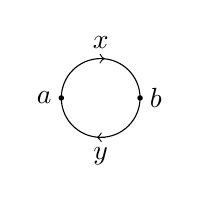
\begin{tikzpicture}[baseline=-4]
            \draw(0,0) circle[radius=0.5];
            \fill (-0.5,0) circle (1pt) node[left] {$a$};
            \fill (0.5,0) circle (1pt) node[right] {$b$};
            \node[above] at (0, 0.5) {$x$};
            \node[below] at (0, -0.5) {$y$};
            \draw[->] (-0.05, 0.5) -- (0.05, 0.5);
            \draw[<-] (-0.05, -0.5) -- (0.05, -0.5);
        \end{tikzpicture}

        Построим $C_0 = \Z a + \Z b$ --- свободная абелева группа на $\{a, b\}$, $C_1 = \Z x + \Z y$ --- тоже свободная абелева группа, но на образующих $\{x, y\}$.
        Вместо $\Z$ можно было взять любое другое кольцо.

        Все остальные элементы комплекса объявляются нулями.
    % https://q.uiver.app/#q=WzAsNCxbMCwwLCIwIl0sWzEsMCwiQ18xIl0sWzIsMCwiQ18wIl0sWzMsMCwiMCJdLFsyLDNdLFsxLDIsImRfMSJdLFswLDFdXQ==
        \[\begin{tikzcd}[ampersand replacement=\&]
              0 \& {C_1} \& {C_0} \& 0
              \arrow[from=1-3, to=1-4]
              \arrow["{d_1}", from=1-2, to=1-3]
              \arrow[from=1-1, to=1-2]
        \end{tikzcd}\]

        Определим $d_1$, как <<конец минус начало>>: $\all{d_1(x) = b - a,\\ d_1(y) = a - b}$.

        Теперь $\all{Z_0 = C_0 \\ Z_1 = \Z(x + y)} \all{B_0 = \Z(b - a) \\ B_1 = 0}$ и $\all{H_0 = Z_0 / B_0 = (\Z a + \Z b)/\Z(b - a) &\cong \Z \\ H_1 = Z_1/B_1 = \Z(x + y) &\cong \Z}$.
        \item Теперь триангулируем окружность по-другому:
        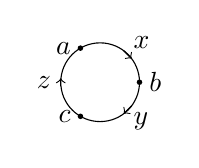
\begin{tikzpicture}[baseline=-4]
            \draw(0,0) circle[radius=0.5];
            \fill (-0.25,0.433) circle (1pt) node[left] {$a$};
            \fill (-0.25,-0.433) circle (1pt) node[left] {$c$};
            \fill (0.5,0) circle (1pt) node[right] {$b$};
            \node[above,right] at (0.3, 0.5) {$x$};
            \node[below,right] at (0.3, -0.5) {$y$};
            \node[left] at (-0.5, 0) {$z$};
            \draw[->] (-0.5, -0.05) -- (-0.5, 0.05);
            \draw[->] (0.3, 0.4) -- (0.4, 0.3);
            \draw[->] (0.4, -0.3) -- (0.3, -0.4);
        \end{tikzpicture}
        $\all{d_1(x) = b - a,\\ d_1(y) = c - b,\\ d_1(z) =  a - c}$.

        Теперь $\all{Z_0 = C_0 \\ Z_1 = \Z(x + y + z)}$, $\all{B_0 = \Z(b - a) + \Z(c - b) \\ B_1 = 0}$ и $\all{H_0  &\cong \Z \\ H_1 = \Z(x + y + z)/0 &\cong \Z}$.
    }
    Ответ получился тот же самый, и это не случайно --- есть теорема, что сингулярные/симплициальные гомологии (они равны для клеточных пространств) не зависят от триангуляции.
    \exercise{
        Триангулировать сферу, и вычислить гомологии. Дифференциал от треугольника $ABC$ (ориентация --- порядок вершин --- важна) определяют, как его обход вдоль периметра: $AB + BC + CA$.
    }

    \theorem[Длинная точная последовательность гомологий]{
        Пусть имеется точная последовательность комплексов $0 \map A' \map A \map A'' \map 0$.

        Существует длинная точная последовательность гомологических групп
    % https://q.uiver.app/#q=WzAsNyxbMCwwLCJcXGNkb3RzIl0sWzEsMCwiSCciXSxbMiwwLCJIIl0sWzMsMCwiSCcnIl0sWzQsMCwiSCdbLTFdIl0sWzUsMCwiSFstMV0iXSxbNiwwLCJcXGNkb3RzIl0sWzAsMV0sWzEsMl0sWzIsM10sWzMsNF0sWzQsNV0sWzUsNl1d
        \[\begin{tikzcd}[ampersand replacement=\&]
              \cdots \& {H'} \& H \& {H''} \& {H'[-1]} \& {H[-1]} \& \cdots
              \arrow[from=1-1, to=1-2]
              \arrow[from=1-2, to=1-3]
              \arrow[from=1-3, to=1-4]
              \arrow[from=1-4, to=1-5]
              \arrow[from=1-5, to=1-6]
              \arrow[from=1-6, to=1-7]
        \end{tikzcd}\]
        где связующий морфизм $\delta$ будет построен в доказательстве.

        Более того, это всё функториально: если есть другая короткая точная последовательность, и морфизм между ними, то по отношению к ним найдётся естественный морфизм полученных длинных точных последовательностей гомологий.
        \provehere{
            Сначала строим $\delta$.

            Для $z \in Z_n''$, обозначим за $[z]$ класс $z$ в $H_n''$.
        % https://q.uiver.app/#q=WzAsMTAsWzAsMCwiMCJdLFsxLDAsIkFfbiciXSxbMiwwLCJBX24iXSxbMywwLCJBX24nJyJdLFs0LDAsIjAiXSxbMCwxLCIwIl0sWzEsMSwiQV97bi0xfSciXSxbMiwxLCJBX3tuLTF9Il0sWzMsMSwiQScnX3tuLTF9Il0sWzQsMSwiMCJdLFsyLDMsIlxccGkiXSxbMiw3LCJkIl0sWzYsNywiaSJdLFs3LDhdLFs4LDldLFszLDRdLFszLDgsImQnJyJdLFsxLDJdLFsxLDYsImQnIl0sWzAsMV0sWzUsNl1d
            \[\begin{tikzcd}[ampersand replacement=\&]
                  0 \& {A_n'} \& {A_n} \& {A_n''} \& 0 \\
                  0 \& {A_{n-1}'} \& {A_{n-1}} \& {A''_{n-1}} \& 0
                  \arrow["\pi", from=1-3, to=1-4]
                  \arrow["d", from=1-3, to=2-3]
                  \arrow["i", from=2-2, to=2-3]
                  \arrow[from=2-3, to=2-4]
                  \arrow[from=2-4, to=2-5]
                  \arrow[from=1-4, to=1-5]
                  \arrow["{d''}", from=1-4, to=2-4]
                  \arrow[from=1-2, to=1-3]
                  \arrow["{d'}", from=1-2, to=2-2]
                  \arrow[from=1-1, to=1-2]
                  \arrow[from=2-1, to=2-2]
            \end{tikzcd}\]
            Положим $\delta([z]) \coloneqq [i^{-1}(d(\pi^{-1}(z)))]$, где $\pi^{-1}(z)$ --- произвольный прообраз (он есть, так как $\pi$ сюръективно).

            \comment{
                Дальше надо проверить, что определение корректно, и последовательность точна.
                Это типичный диаграммный поиск, который невозможно записывать, и его несложно воспроизвести самостоятельно.
            }
        }
    }
    \newlection{4 марта 2024 г.}
    Теперь приведём другое доказательство существования длинной точной последовательности гомологий, опирающееся на лемму о змее.
    \lemma[О змее]{
        Пусть даны два комплекса $A' \map A \map A'' \map 0$ и $0 \map B' \map B \map B''$, и морфизм между ними.
        Тогда имеется длинная точная последовательность из пунктирных стрелок.

        Короткие стрелки получены из действия соответственных функторов (ядра и коядра), а связующий гомоморфизм определён $\delta$ определён в доказательстве, и естественен (функториален).
    % https://q.uiver.app/#q=WzAsMTQsWzEsMSwiQSciXSxbMiwxLCJBIl0sWzMsMSwiQScnIl0sWzQsMSwiMCJdLFswLDIsIjAiXSxbMSwyLCJCJyJdLFsyLDIsIkIiXSxbMywyLCJCJyciXSxbMSwwLCJcXEtlciBcXHBoaSciXSxbMiwwLCJcXEtlciBcXHBoaSJdLFszLDAsIlxcS2VyIFxccGhpJyciXSxbMSwzLCJcXENvS2VyIFxccGhpJyJdLFsyLDMsIlxcQ29LZXIgXFxwaGkiXSxbMywzLCJcXENvS2VyXFxwaGknJyJdLFsyLDcsIlxccGhpJyciXSxbMSw2LCJcXHBoaSJdLFswLDUsIlxccGhpIl0sWzQsNV0sWzUsNl0sWzYsN10sWzAsMV0sWzEsMl0sWzIsM10sWzgsMCwiXFxrZXIgXFxwaGknIl0sWzksMSwiXFxrZXIgXFxwaGkiXSxbMTAsMiwiXFxrZXIgXFxwaGknJyJdLFs1LDExLCJcXGNva2VyIFxccGhpJyJdLFs2LDEyLCJcXGNva2VyIFxccGhpIl0sWzcsMTMsIlxcY29rZXIgXFxwaGknJyJdLFs4LDksIiIsMSx7InN0eWxlIjp7ImJvZHkiOnsibmFtZSI6ImRhc2hlZCJ9fX1dLFs5LDEwLCIiLDEseyJzdHlsZSI6eyJib2R5Ijp7Im5hbWUiOiJkYXNoZWQifX19XSxbMTEsMTIsIiIsMSx7InN0eWxlIjp7ImJvZHkiOnsibmFtZSI6ImRhc2hlZCJ9fX1dLFsxMiwxMywiIiwxLHsic3R5bGUiOnsiYm9keSI6eyJuYW1lIjoiZGFzaGVkIn19fV1d
        \[\begin{tikzcd}[ampersand replacement=\&]
              \& {\Ker \phi'} \& {\Ker \phi} \& {\Ker \phi''} \\
              \& {A'} \& A \& {A''} \& 0 \\
              0 \& {B'} \& B \& {B''} \\
              \& {\CoKer \phi'} \& {\CoKer \phi} \& {\CoKer\phi''}
              \arrow["{\phi''}", from=2-4, to=3-4]
              \arrow["\phi", from=2-3, to=3-3, ""{coordinate, near start, name=Z}]
              \arrow["\phi", from=2-2, to=3-2]
              \arrow[from=3-1, to=3-2]
              \arrow[from=3-2, to=3-3]
              \arrow[from=3-3, to=3-4]
              \arrow[from=2-2, to=2-3]
              \arrow[from=2-3, to=2-4]
              \arrow[from=2-4, to=2-5]
              \arrow["{\ker \phi'}", from=1-2, to=2-2]
              \arrow["{\ker \phi}", from=1-3, to=2-3]
              \arrow[dll, "\delta", dashed, rounded corners, to path={ -- ([xshift=10ex]\tikztostart.east) |- (Z) \tikztonodes -| ([xshift=-10ex]\tikztotarget.west)-- (\tikztotarget)},from=1-4,to=4-2]
              \arrow["{\ker \phi''}", from=1-4, to=2-4]
              \arrow["{\coker \phi'}", from=3-2, to=4-2]
              \arrow["{\coker \phi}", from=3-3, to=4-3]
              \arrow["{\coker \phi''}", from=3-4, to=4-4]
              \arrow[dashed, from=1-2, to=1-3]
              \arrow[dashed, from=1-3, to=1-4]
              \arrow[dashed, from=4-2, to=4-3]
              \arrow[dashed, from=4-3, to=4-4]
        \end{tikzcd}\]
        \provehere{
            Диаграммный поиск.
        }
    }

    \theorem[Длинная точная последовательность гомологий на бис]{
        Пусть имеется точная последовательность комплексов $0 \map A' \map A \map A'' \map 0$.

        Существует длинная точная последовательность гомологических групп
    % https://q.uiver.app/#q=WzAsNyxbMCwwLCJcXGNkb3RzIl0sWzEsMCwiSCciXSxbMiwwLCJIIl0sWzMsMCwiSCcnIl0sWzQsMCwiSCdbLTFdIl0sWzUsMCwiSFstMV0iXSxbNiwwLCJcXGNkb3RzIl0sWzAsMV0sWzEsMl0sWzIsM10sWzMsNF0sWzQsNV0sWzUsNl1d
        \[\begin{tikzcd}[ampersand replacement=\&]
              \cdots \& {H'} \& H \& {H''} \& {H'[-1]} \& {H[-1]} \& \cdots
              \arrow[from=1-1, to=1-2]
              \arrow[from=1-2, to=1-3]
              \arrow[from=1-3, to=1-4]
              \arrow[from=1-4, to=1-5]
              \arrow[from=1-5, to=1-6]
              \arrow[from=1-6, to=1-7]
        \end{tikzcd}\]
        где связующий морфизм $\delta$ будет построен в доказательстве.

        Более того, это всё функториально.
        \provehere{
            Длинная точная последовательность комплексов означает наличие следующей коммутативной диаграммы (где строки точны, и столбцы --- комплексы)
        % https://q.uiver.app/#q=WzAsMTYsWzEsMSwiQV9uJyJdLFsyLDEsIkFfbiJdLFszLDEsIkFfbicnIl0sWzQsMSwiMCJdLFswLDIsIjAiXSxbMSwyLCJBX3tuLTF9JyJdLFsyLDIsIkFfe24tMX0iXSxbMywyLCJBJydfe24tMX0iXSxbMCwxLCIwIl0sWzQsMiwiMCJdLFsxLDAsIlxcdmRvdHMiXSxbMiwwLCJcXHZkb3RzIl0sWzMsMCwiXFx2ZG90cyJdLFsxLDMsIlxcdmRvdHMiXSxbMiwzLCJcXHZkb3RzIl0sWzMsMywiXFx2ZG90cyJdLFswLDFdLFsxLDJdLFsyLDNdLFs0LDVdLFs1LDZdLFs2LDddLFswLDUsImQnX24iXSxbMSw2LCJkX24iXSxbMiw3LCJkJydfbiJdLFs4LDBdLFs3LDldLFsxMCwwXSxbMTEsMV0sWzEyLDJdLFs1LDEzXSxbNiwxNF0sWzcsMTVdXQ==
            \[\begin{tikzcd}[ampersand replacement=\&]
                  \& \vdots \& \vdots \& \vdots \\
                  0 \& {A_n'} \& {A_n} \& {A_n''} \& 0 \\
                  0 \& {A_{n-1}'} \& {A_{n-1}} \& {A''_{n-1}} \& 0 \\
                  \& \vdots \& \vdots \& \vdots
                  \arrow[from=2-2, to=2-3]
                  \arrow[from=2-3, to=2-4]
                  \arrow[from=2-4, to=2-5]
                  \arrow[from=3-1, to=3-2]
                  \arrow[from=3-2, to=3-3]
                  \arrow[from=3-3, to=3-4]
                  \arrow["{d'_n}", from=2-2, to=3-2]
                  \arrow["{d_n}", from=2-3, to=3-3]
                  \arrow["{d''_n}", from=2-4, to=3-4]
                  \arrow[from=2-1, to=2-2]
                  \arrow[from=3-4, to=3-5]
                  \arrow[from=1-2, to=2-2]
                  \arrow[from=1-3, to=2-3]
                  \arrow[from=1-4, to=2-4]
                  \arrow[from=3-2, to=4-2]
                  \arrow[from=3-3, to=4-3]
                  \arrow[from=3-4, to=4-4]
            \end{tikzcd}\]
            Пусть циклы, границы и гомологии в комплексе $A$ обозначаются $Z_\bullet, B_\bullet, H_\bullet$ соответственно, в $A'$ --- $Z_\bullet', B_\bullet', H_\bullet'$, , в $A'$ --- $Z_\bullet'', B_\bullet'', H_\bullet''$.
            Из коммутативности диаграммы $B'_n$ вправо уходит в $B_n$, а $B_n$, в свою очередь --- в $B_n''$.

            Чтобы воспользоваться леммой о змее, построим следующую диаграмму, взяв коядро верхней строки, ядро --- нижней, и дорисовав сверху --- ядра вертикальных стрелок, снизу --- коядра.
% https://q.uiver.app/#q=WzAsMTQsWzEsMSwiQSdfbi9CJ19uIl0sWzIsMSwiQV9uL0JfbiJdLFszLDEsIkFfbicnL0JfbicnIl0sWzQsMSwiMCJdLFswLDIsIjAiXSxbMSwyLCJaX3tuLTF9JyJdLFsyLDIsIlpfe24tMX0iXSxbMywyLCJaJydfe24tMX0iXSxbMSwwLCJIX24nIl0sWzIsMCwiSF9uIl0sWzMsMCwiSCcnX24iXSxbMSwzLCJIX3tuLTF9JyJdLFsyLDMsIkhfe24tMX0iXSxbMywzLCJIX3tuLTF9JyciXSxbMCwxXSxbMSwyXSxbMiwzXSxbNCw1XSxbNSw2XSxbNiw3XSxbMCw1LCJcXG92ZXJsaW5le2R9J19uIl0sWzEsNiwiXFxvdmVybGluZXtkfV9uIl0sWzIsNywiXFxvdmVybGluZXtkfScnX24iXSxbOCwwXSxbOSwxXSxbMTAsMl0sWzUsMTFdLFs2LDEyXSxbNywxM11d
            \[\begin{tikzcd}[ampersand replacement=\&]
                  \& {H_n'} \& {H_n} \& {H''_n} \\
                  \& {A'_n/B'_n} \& {A_n/B_n} \& {A_n''/B_n''} \& 0 \\
                  0 \& {Z_{n-1}'} \& {Z_{n-1}} \& {Z''_{n-1}} \\
                  \& {H_{n-1}'} \& {H_{n-1}} \& {H_{n-1}''}
                  \arrow[from=2-2, to=2-3]
                  \arrow[from=2-3, to=2-4]
                  \arrow[from=2-4, to=2-5]
                  \arrow[from=3-1, to=3-2]
                  \arrow[from=3-2, to=3-3]
                  \arrow[from=3-3, to=3-4]
                  \arrow["{\overline{d}'_n}", from=2-2, to=3-2]
                  \arrow["{\overline{d}_n}", from=2-3, to=3-3]
                  \arrow["{\overline{d}''_n}", from=2-4, to=3-4]
                  \arrow[from=1-2, to=2-2]
                  \arrow[from=1-3, to=2-3]
                  \arrow[from=1-4, to=2-4]
                  \arrow[from=3-2, to=4-2]
                  \arrow[from=3-3, to=4-3]
                  \arrow[from=3-4, to=4-4]
            \end{tikzcd}\]
            Обоснуем, каким образом получилась такая диаграмма.
            По определению $d_n(B_n) = \{0\}$, поэтому $A_n \overset{d_n}\Map A_{n-1}$ пропускается через фактор, и получается отображение $\tilde{d}_n: A_n/B_n \map A_{n-1}$.
            Так как $A$ --- комплекс, то $\tilde{d}_n(A_n/B_n) \subset Z_{n-1}$, можно сузить codomain, получая $\overline{d}_n$.
            По определению $H_n = Z_n/B_n$, поэтому действительно $H_n = \Ker(d_n)$.
            В свою очередь, $H_{n-1} = Z_{n-1}/B_{n-1}$, и это действительно $\CoKer(d_n)$.

            Отображение $A_n \map A_n''$ было эпиморфизмом, после взятия коядра эпиморфизмом оно и осталось.
            Двойственно, $A'_{n-1} \map A_{n-1}$ было мономорфизмом, мономорфизмом оно и осталось.

            Применяя лемму о змее, получаем утверждение теоремы.
        }
    }


    \section{Функторы между абелевыми категориями}
    Пусть $\cat A, \cat B$ --- абелевы категории.
    \definition[Аддитивный функтор $\cat F: \cat A \map \cat B$]{
        Такой функтор, что $\forall \alpha, \beta \in \Mor(\cat A): \cat F(\alpha + \beta) = \cat F(\alpha) + \cat F(\beta)$ всегда, когда определено.
    }
    Рассмотрим произвольную короткую точную последовательность $0 \map A' \map A \map A'' \map 0$ в $\cat A$.
    Подействовав на неё функтором $\cat F$, мы получим последовательность $0 \map \cat F(A') \map \cat F(A) \map \cat F(A'') \map 0$.
    Точность, вообще говоря, пропадёт, но если $\cat F$ сохраняет точность в каком-то члене для всех таких коротких точных последовательностей, то функтор $\cat F$ имеет соответствующее название:
    \numbers{
        \item Если всегда имеется точность в члене $\cat F(A)$, то $\cat F$ --- \emph{полуточный функтор}.
        \item Если всегда имеется точность в членах $\cat F(A')$ и $\cat F(A)$, то $\cat F$ --- \emph{точный слева функтор}.
        \item Если всегда имеется точность в членах $\cat F(A)$ и $\cat F(A'')$, то $\cat F$ --- \emph{точный справа функтор}.
        \item Если всякая короткая точная последовательность переходит в короткую точную последовательность, то $\cat F$ --- \emph{точный функтор}.
    }
    \lemma{
        Пусть $\cat F$ --- аддитивный функтор. Следующие условия эквивалентны:
        \numbers{
            \item $\cat F$ точен справа.
            \item $\cat F$ сохраняет нуль и коядра: $\cat F(0) = 0, \cat F(\coker(\phi)) = \coker(\cat F(\phi))$.
            \item $\cat F$ сохраняет конечные копределы.
        }
        \provebullets{
            \item[$(3)\then(2)$] Коядро --- конечный копредел, поэтому очевидно.
            \item[$(2)\then(3)$] В свою очередь, копроизведение в абелевой категории --- бипроизведение, а это <<внутренний объект>>, поэтому всякий аддитивный функтор сохраняет его.
            \item[$(2)\then(1)$] Короткая точная последовательность $A' \overset{\phi}\map A \overset{\psi}\map A'' \map 0$ характеризуется свойствами $\psi = \coker \phi, 0 = \coker \psi$.
            \item[$(1) \then (2)$] Рассмотрим произвольный $\phi: A' \map A$.
            У него есть эпи-моно разложение $\phi = \mu\eps$ ($\mu$ --- моно, $\eps$ --- эпи), и $\coker(\mu\eps) = \coker(\mu)$, так как $\eps$ --- эпиморфизм.
            Значит, без потери общности $\phi$ --- мономорфизм.

            Тогда последовательность $0 \map A' \overset{\phi}\map A \overset{\coker \phi}\map \CoKer\phi \map 0$ точна, и так как $\cat F$ --- точен справа, то $\cat F(\coker \phi) = \coker(\cat F(\phi))$.

            Также точный справа функтор сохраняет нуль: $0 \map A \overset{\id}\map A \map 0 \map 0$ переходит в $\cat F(A) \overset{\id}\map \cat F(A) \map \cat F(0) \map 0$.
        }
    }
    \corollary{
        Левый сопряжённый функтор точен справа.
        \provehere{Он сохраняет копределы.}
    }
    Копредел (который является левым сопряжённым к диагональному $\Delta$) сохраняет копределы, значит, точен справа.
    Другими словами, копределы коммутируют.

    К сожалению, в лемме о змее это не помогает в доказательстве того, что последовательность точна в члене $\Ker \phi$, так как нет точной последовательности $0 \map A' \map A \map A'' \map 0$.

    При доказательстве существования длинной точной последовательности гомологий на бис, мы использовали, что коядро точно справа, ядро --- точно слева.
    \newlection{11 марта 2024 г.}

    \fact{
        Если точный справа функтор сохраняет мономорфизмы, то функтор точен.
        Двойственно, точный слева функтор, сохраняющий эпиморфизмы, точен.
        \provehere{
            Условия как раз означают, что короткая точная последовательность отображается в короткую точную последовательность.
        }
    }
    Пусть имеются комплексы $X_\bullet$ и $X'_\bullet$, и между ними морфизмы $f, g$.
    \definition[Морфизмы $f$ и $g$ гомотопны]{
        Существует семейство морфизмов $s_k: X_{k-1} \map X'_k$, таких, что $f_{n} - g_{n} = d'_{n}s_{n+1} + s_{n}d_{n-1}$.
        При этом диаграмма ниже \textbf{не обязана} быть коммутативной.
        % https://q.uiver.app/#q=WzAsMTAsWzEsMCwiWF9uIl0sWzIsMCwiWF97bi0xfSJdLFszLDAsIlxcY2RvdHMiXSxbNCwwLCJYXzAiXSxbMSwxLCJYJ19uIl0sWzIsMSwiWCdfe24tMX0iXSxbMywxLCJcXGNkb3RzIl0sWzQsMSwiWCdfMCJdLFswLDEsIlgnX3tuKzF9Il0sWzAsMCwiWF97bisxfSJdLFswLDQsImZfbiIsMix7ImxhYmVsX3Bvc2l0aW9uIjo4MCwib2Zmc2V0IjoxfV0sWzAsNCwiZ19uIiwwLHsibGFiZWxfcG9zaXRpb24iOjIwLCJvZmZzZXQiOi0xfV0sWzEsNSwiZl97bi0xfSIsMix7ImxhYmVsX3Bvc2l0aW9uIjo4MCwib2Zmc2V0IjoxfV0sWzEsNSwiZ197bi0xfSIsMCx7ImxhYmVsX3Bvc2l0aW9uIjoyMCwib2Zmc2V0IjotMX1dLFszLDcsImZfMCIsMix7ImxhYmVsX3Bvc2l0aW9uIjo4MCwib2Zmc2V0IjoxfV0sWzMsNywiZ18wIiwwLHsibGFiZWxfcG9zaXRpb24iOjIwLCJvZmZzZXQiOi0xfV0sWzAsMSwiZF97bi0xfSJdLFsxLDIsImRfe24tMn0iXSxbMiwzLCJkXzAiXSxbNiw3LCJkJ18wIiwyXSxbNSw2LCJkJ197bi0yfSIsMl0sWzQsNSwiZCdfe24tMX0iLDJdLFs4LDQsImQnX3tufSIsMl0sWzksOCwiZl97bisxfSIsMix7ImxhYmVsX3Bvc2l0aW9uIjo4MCwib2Zmc2V0IjoxfV0sWzksOCwiZ197bisxfSIsMCx7ImxhYmVsX3Bvc2l0aW9uIjoyMCwib2Zmc2V0IjotMX1dLFs5LDAsImRfe259Il0sWzgsMCwic197bisxfSIsMyx7InN0eWxlIjp7InRhaWwiOnsibmFtZSI6ImFycm93aGVhZCJ9LCJib2R5Ijp7Im5hbWUiOiJkb3R0ZWQifSwiaGVhZCI6eyJuYW1lIjoibm9uZSJ9fX1dLFs0LDEsInNfbiIsMyx7InN0eWxlIjp7InRhaWwiOnsibmFtZSI6ImFycm93aGVhZCJ9LCJib2R5Ijp7Im5hbWUiOiJkb3R0ZWQifSwiaGVhZCI6eyJuYW1lIjoibm9uZSJ9fX1dLFs1LDIsInNfe24tMX0iLDMseyJzdHlsZSI6eyJ0YWlsIjp7Im5hbWUiOiJhcnJvd2hlYWQifSwiYm9keSI6eyJuYW1lIjoiZG90dGVkIn0sImhlYWQiOnsibmFtZSI6Im5vbmUifX19XSxbNiwzLCJzXzEiLDMseyJzdHlsZSI6eyJ0YWlsIjp7Im5hbWUiOiJhcnJvd2hlYWQifSwiYm9keSI6eyJuYW1lIjoiZG90dGVkIn0sImhlYWQiOnsibmFtZSI6Im5vbmUifX19XV0=
        \[\begin{tikzcd}[ampersand replacement=\&]
        {X_{n+1}}
              \& {X_n} \& {X_{n-1}} \& \cdots \& {X_0} \\
              {X'_{n+1}} \& {X'_n} \& {X'_{n-1}} \& \cdots \& {X'_0}
              \arrow["{f_n}"'{pos=0.8}, shift right, from=1-2, to=2-2]
              \arrow["{g_n}"{pos=0.2}, shift left, from=1-2, to=2-2]
              \arrow["{f_{n-1}}"'{pos=0.8}, shift right, from=1-3, to=2-3]
              \arrow["{g_{n-1}}"{pos=0.2}, shift left, from=1-3, to=2-3]
              \arrow["{f_0}"'{pos=0.8}, shift right, from=1-5, to=2-5]
              \arrow["{g_0}"{pos=0.2}, shift left, from=1-5, to=2-5]
              \arrow["{d_{n-1}}", from=1-2, to=1-3]
              \arrow["{d_{n-2}}", from=1-3, to=1-4]
              \arrow["{d_0}", from=1-4, to=1-5]
              \arrow["{d'_0}"', from=2-4, to=2-5]
              \arrow["{d'_{n-2}}"', from=2-3, to=2-4]
              \arrow["{d'_{n-1}}"', from=2-2, to=2-3]
              \arrow["{d'_{n}}"', from=2-1, to=2-2]
              \arrow["{f_{n+1}}"'{pos=0.8}, shift right, from=1-1, to=2-1]
              \arrow["{g_{n+1}}"{pos=0.2}, shift left, from=1-1, to=2-1]
              \arrow["{d_{n}}", from=1-1, to=1-2]
              \arrow["{s_{n+1}}"{marking, allow upside down}, dotted, tail reversed, no head, from=2-1, to=1-2]
              \arrow["{s_n}"{marking, allow upside down}, dotted, tail reversed, no head, from=2-2, to=1-3]
              \arrow["{s_{n-1}}"{marking, allow upside down}, dotted, tail reversed, no head, from=2-3, to=1-4]
              \arrow["{s_1}"{marking, allow upside down}, dotted, tail reversed, no head, from=2-4, to=1-5]
        \end{tikzcd}\]
        Пишут $f \simeq g$.
    }
    \comment{А почему это то же самое, что и гомотопность в топологии?}
    \theorem{\label{homotopy-preserves-h}
    Если два морфизма комплексов $f, g: X \map X'$ гомотопны, то $H(f) = H(g)$ (гомологии являются функтором, и действуют не только на комплексах, но и на морфизмах между ними).
    \provehere{
        Докажем, что $H(f - g) = 0$.

        Рассмотрим $\overline{x} \in H_n(X)$.
        У него имеется прообраз $x \in Z_n$.

        Заметим, что $H(f_n - g_n)(\overline{x}) = \overline{(f_n - g_n)(x)} = \overline{d'_n(s_{n+1}(x))} + \overline{s_n(d_{n-1}(x))}$.
        Первое слагаемое равно нулю, так как $d'_n(\cdots) \in B_n(X')$, а второе --- так как $x \in \Ker d_{n-1}$.
    }
    }
    \note{
        Если $\cat F: \cat A \map \cat A$ --- аддитивный функтор, и $f \simeq g$ --- морфизмы комплексов с объектами из $\cat A$, то (допуская вольность речи можно писать $\cat F(f)$) $\cat F(f) \simeq \cat F(g)$.
    }
    \fact{
        Быть гомотопными --- отношение эквивалентности.
        \provehere{
            Рефлексивность: $\forall n: s_n = 0$.
            Симметричность: $s_n \coloneqq -s_n$.
            Транзитивность: \[\all{f_n - g_n = d'_n s_{n+1} + s_n d_{n-1} \\ g_n - h_n =d'_n r_{n+1} + r_n d_{n-1}} \then f_n - h_n = d'_n(s_{n+1} + r_{n+1}) + (s_n + r_n)d_{n-1}\qedhere\]
        }
    }
    \definition[Два комплекса $X$ и $X'$ гомотопически эквивалентны]{
        Существуют морфизмы комплексов $f: X \map X'$ и $g: X' \map X$, такие, что $f g \simeq \id_{X'}$ и $g f \simeq \id_{X}$.
        Данные морфизмы $f$ и $g$ называют \emph{гомотопическими эквивалентностями}.
    }
    \fact{
        Если $X$ и $X'$ гомотопически эквивалентны, то $H(X) \cong H(X')$.
    }
    \definition[Квазиизоморфизм $f: X \map X'$]{
        Морфизм $f$, такой, что $H(f)$ --- изоморфизм.
    }
    \fact{
        Гомотопическая эквивалентность --- квазиизоморфизм.
    }
    \definition[Комплекс $X$ ацикличен]{
        $X$ точен, то есть $H(X) = 0$.
    }
    \definition[Комплекс $X$ стягиваем]{
        $\id_X \simeq 0_X$.
    }
    \note{
        Из~(\cref{homotopy-preserves-h}) следует, что стягиваемый комплекс ацикличен.
    }
    Обратное, вообще говоря, неверно.
    Стягиваемый комплекс сохраняется под действием функторов, а ацикличный --- может и не сохраниться.


    \section{Резольвенты}
%    \subsection{Идея}
%    Пусть имеется точный комплекс $\cdots \map P_2 \map P_1 \map P_0 \map M \map 0$, где $P_i$ --- свободные модули.
%
%    Применяя $\cat F$, получим комплекс $\cdots \map \cat F(P_1) \map \cat F(P_0) \map \cat F(M) \map 0$.
%    Определим $L_n\cat F(M) \bydef H_n(X)$.
%    \comment{Я не понял.}
%    \ok
    Пусть $\cat A$ --- абелева категория, $P \in \cat A$.
    \definition[Объект $P$ проективен]{
        $\forall \phi: A \map B$: $\phi$ --- эпи $\then \forall \psi: P \map B$: $\exists {\theta: P \map A}$, причём диаграмма коммутирует.
        При этом $\theta$ должно найтись какое-то, не факт, что оно единственно.
        % https://q.uiver.app/#q=WzAsNCxbMCwxLCJBIl0sWzEsMSwiQiJdLFsyLDEsIjAiXSxbMSwwLCJQIl0sWzAsMSwiXFxmb3JhbGwgXFxwaGkiXSxbMSwyXSxbMywxLCJcXGZvcmFsbCBcXHBzaSJdLFszLDAsIlxcZXhpc3RzIFxcdGhldGEiLDJdXQ==
        \[\begin{tikzcd}[ampersand replacement=\&]
              \& P \\
              A \& B \& 0
              \arrow["{\forall \phi}", from=2-1, to=2-2]
              \arrow[from=2-2, to=2-3]
              \arrow["{\forall \psi}", from=1-2, to=2-2]
              \arrow["{\exists \theta}"', from=1-2, to=2-1]
        \end{tikzcd}\]
    }
    \fact{
        В $\cat{Set}$ все множества --- проективные объекты.
    }
    \theorem{
        Пусть $\cat A = \Lmod{R}$.
        Модуль $P$ проективен $\iff$ $P$ является прямым слагаемым свободного модуля.
        \provenumbers{
            \item Свободный модуль проективен: пусть $\{p_\alpha\}$ --- базис $P$. Определим $\theta(p_\alpha) = \psi(\phi^{-1}(p_\alpha))$, где прообраз выбран произвольно, и продолжим по линейности.
            \item Прямое слагаемое проективного модуля проективно.
            Рассмотрим каноническое вложение $M \hookrightarrow M \oplus N$, где $M \oplus N$ --- проективен.
        % https://q.uiver.app/#q=WzAsNSxbMSwwLCJNIl0sWzIsMCwiTVxcb3BsdXMgTiJdLFsxLDEsIkIiXSxbMCwxLCJBIl0sWzIsMSwiMCJdLFszLDIsIiIsMCx7InN0eWxlIjp7ImhlYWQiOnsibmFtZSI6ImVwaSJ9fX1dLFsyLDRdLFswLDFdLFsxLDIsIiIsMCx7InN0eWxlIjp7ImJvZHkiOnsibmFtZSI6ImRhc2hlZCJ9fX1dLFsxLDMsIiIsMCx7ImN1cnZlIjo0fV0sWzAsMiwiXFxwc2kiXV0=
            \[\begin{tikzcd}[ampersand replacement=\&]
                  \& M \& {M\oplus N} \\
                  A \& B \& 0
                  \arrow[two heads, from=2-1, to=2-2]
                  \arrow[from=2-2, to=2-3]
                  \arrow[from=1-2, to=1-3]
                  \arrow[dashed, from=1-3, to=2-2]
                  \arrow[curve={height=36pt}, from=1-3, to=2-1]
                  \arrow["\psi", from=1-2, to=2-2]
            \end{tikzcd}\]
            Определим $M \oplus N \map B, (m, n) \mapsto \psi(m)$.
            Так как $M \oplus N$ проективен, то найдётся $M \oplus N \map A$, и композиция $M \map M \oplus N \map A$ подходит в качестве морфизма, который должен найтись из определения проективного модуля.
            \item Пусть $P$ проективен. Возьмём свободный модуль $F$, сюръективно накрывающий $P$ (например, подойдёт свободный модуль на всех элементах $P$, но на практике, конечно, удобно брать модуль поменьше).
        % https://q.uiver.app/#q=WzAsMyxbMSwwLCJQIl0sWzEsMSwiUCJdLFswLDEsIkYiXSxbMiwxLCJcXHBpIiwwLHsic3R5bGUiOnsiaGVhZCI6eyJuYW1lIjoiZXBpIn19fV0sWzAsMSwiXFxpZCIsMl0sWzAsMiwiXFxleGlzdHMiLDIseyJzdHlsZSI6eyJib2R5Ijp7Im5hbWUiOiJkYXNoZWQifX19XV0=
            \[\begin{tikzcd}[ampersand replacement=\&]
                  \& P \\
                  F \& P
                  \arrow["\pi", two heads, from=2-1, to=2-2]
                  \arrow["\id"', from=1-2, to=2-2]
                  \arrow["\exists"', dashed, from=1-2, to=2-1]
            \end{tikzcd}\]
            Так как модуль проективен, то найдётся пунктирная стрелка. Значит, $F \cong P \oplus \Ker \pi$
            ($\forall f \in F: \pi^{-1}(f) = P(f) + \Ker \pi$).
        }
    }
    \examples{
        \item Пусть $R = \Z/6\Z$. Тогда $\Z/6\Z$ является $R$-модулем, но $\Z/6\Z \cong \Z/2\Z \oplus \Z/3\Z$, значит, модули $\Z/2\Z$, $\Z/3\Z$, $\Z/6\Z$ все проективны.
        \item Можно предъявить проективный модуль, исходя из топологического факта о том, что шар нельзя причесать.
    }
    \definition[Проективная резольвента модуля $M$]{
        Ацикличный комплекс вида\\ $\cdots \map P_n \map P_{n-1} \map \cdots \map P_0 \map M \map 0$, где $P_i$ --- проективные модули.
    }
    В будущем докажем, что любые две проективные резольвенты гомотопически эквивалентны.

    \definition[В категории $\cat A$ достаточно много проективных объектов]{
        $\forall A \in \cat A$ найдётся проективный объект $P \in \cat A$ вместе с эпиморфизмом $P \twoheadrightarrow A$.
    }
    Если в нашей категории $\cat A$ достаточно много проективных объектов, то у всякого модуля $M$ найдётся резольвента --- надо просто подряд накрывать возникающие ядра.
    \newlection{18 марта 2024 г.}


    \section{Резольвенты. Левый производный функтор}
    Зафиксируем некоторый аддитивный функтор $\cat F: \cat A \map \cat B$, который обычно будет точен справа.
    Пусть у объекта $A \in \cat A$ имеется проективная резольвента, которую я выделил стрелками $\rightsquigarrow$ .
    % https://q.uiver.app/#q=WzAsOCxbMCwwLCJcXGNkb3RzIl0sWzEsMCwiUF8xIl0sWzIsMCwiUF8wIl0sWzMsMCwiMCJdLFsyLDEsIkEiXSxbMywxLCIwIl0sWzEsMSwiMCJdLFswLDEsIlxcY2RvdHMiXSxbMCwxLCIiLDAseyJzdHlsZSI6eyJib2R5Ijp7Im5hbWUiOiJzcXVpZ2dseSJ9fX1dLFsxLDIsIiIsMCx7InN0eWxlIjp7ImJvZHkiOnsibmFtZSI6InNxdWlnZ2x5In19fV0sWzIsM10sWzIsNCwiIiwwLHsic3R5bGUiOnsiYm9keSI6eyJuYW1lIjoic3F1aWdnbHkifX19XSxbNCw1LCIiLDAseyJzdHlsZSI6eyJib2R5Ijp7Im5hbWUiOiJzcXVpZ2dseSJ9fX1dLFs2LDRdLFs3LDZdXQ==
    \[\begin{tikzcd}[ampersand replacement=\&]
          \cdots \& {P_1} \& {P_0} \& 0 \\
          \cdots \& 0 \& A \& 0
          \arrow[squiggly, from=1-1, to=1-2]
          \arrow[squiggly, from=1-2, to=1-3]
          \arrow[from=1-3, to=1-4]
          \arrow[squiggly, from=1-3, to=2-3]
          \arrow[squiggly, from=2-3, to=2-4]
          \arrow[from=2-2, to=2-3]
          \arrow[from=2-1, to=2-2]
    \end{tikzcd}\]
    Иными словами, проективная резольвента --- это некоторый морфизм комплексов $P$ и $A_\bullet$.
    Под комплексом $A_\bullet$ подразумевается такой комплекс, в котором в нулевой градуировке сидит $A$, а в остальных --- нули (следовательно, все дифференциалы --- тоже нули).

    Раз $\cat F$ точен справа, то он сохраняет нуль.
    Применим $\cat F$ к верхней строчке.
    Тогда получится комплекс вида
    % https://q.uiver.app/#q=WzAsNCxbMCwwLCJcXGNkb3RzIl0sWzEsMCwiXFxjYXQgRihQXzEpIl0sWzIsMCwiXFxjYXQgRihQXzApIl0sWzMsMCwiMCJdLFswLDFdLFsxLDJdLFsyLDNdXQ==
    \[\begin{tikzcd}[ampersand replacement=\&]
          \cdots \& {\cat F(P_1)} \& {\cat F(P_0)} \& 0
          \arrow[from=1-1, to=1-2]
          \arrow[from=1-2, to=1-3]
          \arrow[from=1-3, to=1-4]
    \end{tikzcd}\]
    Чуть ниже мы определим $L_n \cat F(A) \coloneqq H_n \cat F(P)$ --- левый производный функтор, измеряющий неточность $\cat F$ --- но пока, например, неясна корректность (независимость от резольвенты) такого определения.
    \theorem{
        Пусть $P_i$ проективные, сверху комплекс (и ноль в верхней строчке вообще-то неважен), снизу --- точный комплекс.
    % https://q.uiver.app/#q=WzAsMTAsWzEsMCwiUF8xIl0sWzIsMCwiUF8wIl0sWzMsMCwiQSJdLFs0LDAsIjAiXSxbNCwxLCIwIl0sWzMsMSwiQiJdLFsyLDEsIlFfMCJdLFsxLDEsIlFfMSJdLFswLDAsIlxcY2RvdHMiXSxbMCwxLCJcXGNkb3RzIl0sWzgsMF0sWzksN10sWzAsNywiIiwxLHsic3R5bGUiOnsiYm9keSI6eyJuYW1lIjoiZGFzaGVkIn19fV0sWzEsNiwiIiwxLHsic3R5bGUiOnsiYm9keSI6eyJuYW1lIjoiZGFzaGVkIn19fV0sWzIsNSwiZiIsMV0sWzAsMV0sWzEsMl0sWzIsM10sWzUsNF0sWzYsNV0sWzcsNl1d
        \[\begin{tikzcd}[ampersand replacement=\&]
              \cdots \& {P_1} \& {P_0} \& A \& 0 \\
              \cdots \& {Q_1} \& {Q_0} \& B \& 0
              \arrow[from=1-1, to=1-2]
              \arrow[from=2-1, to=2-2]
              \arrow[dashed, from=1-2, to=2-2]
              \arrow[dashed, from=1-3, to=2-3]
              \arrow["f"{description}, from=1-4, to=2-4]
              \arrow[from=1-2, to=1-3]
              \arrow[from=1-3, to=1-4]
              \arrow[from=1-4, to=1-5]
              \arrow[from=2-4, to=2-5]
              \arrow[from=2-3, to=2-4]
              \arrow[from=2-2, to=2-3]
        \end{tikzcd}\]
        Тогда найдутся пунктирные стрелки, и они определены с точностью до гомотопии.
        \provebullets{
            \item\bullets{\item Сначала построим $f_i: P_i \map Q_i$.

                $Q_0 \map B$ сюръективно, значит, найдётся $f_0$, такое, что квадрат коммутативен.

                \item Далее по индукции: пусть построены $f_0, \dots, f_{n}$.
% https://q.uiver.app/#q=WzAsNixbMCwwLCJQX3tuKzF9Il0sWzEsMCwiUF9uIl0sWzIsMCwiUF97bi0xfSJdLFswLDEsIlFfe24rMX0iXSxbMSwxLCJRX24iXSxbMiwxLCJRX3tuLTF9Il0sWzIsNSwiZl97bi0xfSJdLFsxLDQsImZfbiJdLFswLDMsImZfe24rMX0iLDAseyJzdHlsZSI6eyJib2R5Ijp7Im5hbWUiOiJkYXNoZWQifX19XSxbMCwxXSxbMSwyXSxbMyw0XSxbNCw1LCJkXlFfe24tMX0iXV0=
                \[\begin{tikzcd}[ampersand replacement=\&]
                {P_{n+1}}
                      \& {P_n} \& {P_{n-1}} \\
                      {Q_{n+1}} \& {Q_n} \& {Q_{n-1}}
                      \arrow["{f_{n-1}}", from=1-3, to=2-3]
                      \arrow["{f_n}", from=1-2, to=2-2]
                      \arrow["{f_{n+1}}", dashed, from=1-1, to=2-1]
                      \arrow[from=1-1, to=1-2]
                      \arrow[from=1-2, to=1-3]
                      \arrow[from=2-1, to=2-2]
                      \arrow["{d^Q_{n-1}}", from=2-2, to=2-3]
                \end{tikzcd}\]
                Хочется заполучить стрелку $P_{n+1} \map Q_{n+1}$, воспользовавшись проективностью $P_{n+1}$.
                Для этого надо найти сюръективное $Q_{n+1} \map \:?$.
                Так как внизу --- точная последовательность, то $Q_{n+1} \map \Ker (d^Q_{n-1})$ подойдёт: оно сюръективно, так как $P_{n+1} \map P_{n-1}$ нулевой, а квадрат $\begin{tikzcd}[ampersand replacement=\&]
                {P_n}
                                                                                                                                                                                  \& {P_{n-1}} \\
                                                                                                                                                                                  {Q_n} \& {Q_{n-1}}
                                                                                                                                                                                  \arrow[from=1-1, to=1-2]
                                                                                                                                                                                  \arrow[from=1-2, to=2-2]
                                                                                                                                                                                  \arrow[from=2-1, to=2-2]
                                                                                                                                                                                  \arrow[from=1-1, to=2-1]
                \end{tikzcd}$ коммутативен.
                Тем самым, по определению проективного модуля $\exists f_{n+1}$.
            }
            \item\bullets{
                \item Теперь пусть имеются два морфизма комплексов, продолжающих $f$, $f_i$ и $g_i$.
            % https://q.uiver.app/#q=WzAsOSxbMSwwLCJQXzEiXSxbMiwwLCJQXzAiXSxbMywwLCJBIl0sWzEsMSwiUV8xIl0sWzIsMSwiUV8wIl0sWzMsMSwiQiJdLFswLDAsIlxcY2RvdHMiXSxbMCwxLCJcXGNkb3RzIl0sWzQsMSwiMCJdLFswLDFdLFsxLDJdLFs2LDBdLFs3LDNdLFswLDMsImdfMSIsMCx7ImxhYmVsX3Bvc2l0aW9uIjo0MCwib2Zmc2V0IjotMX1dLFswLDMsImZfMSIsMix7Im9mZnNldCI6MX1dLFsxLDQsImdfMCIsMCx7Im9mZnNldCI6LTF9XSxbMSw0LCJmXzAiLDIseyJvZmZzZXQiOjF9XSxbMiw1LCJmIiwxXSxbMyw0XSxbNCw1XSxbNSw4XV0=
                \[\begin{tikzcd}[ampersand replacement=\&]
                      \cdots \& {P_1} \& {P_0} \& A \\
                      \cdots \& {Q_1} \& {Q_0} \& B \& 0
                      \arrow[from=1-2, to=1-3]
                      \arrow[from=1-3, to=1-4]
                      \arrow[from=1-1, to=1-2]
                      \arrow[from=2-1, to=2-2]
                      \arrow["{g_1}"{pos=0.4}, shift left, from=1-2, to=2-2]
                      \arrow["{f_1}"', shift right, from=1-2, to=2-2]
                      \arrow["{g_0}", shift left, from=1-3, to=2-3]
                      \arrow["{f_0}"', shift right, from=1-3, to=2-3]
                      \arrow["f"{description}, from=1-4, to=2-4]
                      \arrow[from=2-2, to=2-3]
                      \arrow[from=2-3, to=2-4]
                      \arrow[from=2-4, to=2-5]
                \end{tikzcd}\]
                Распишем разность: пусть $h_i \coloneqq f_i - g_i$.
                Понятно, что $A \map Q_0$ надо взять нулевым.
            % https://q.uiver.app/#q=WzAsMTAsWzEsMCwiUF8xIl0sWzIsMCwiUF8wIl0sWzMsMCwiQSJdLFsxLDEsIlFfMSJdLFsyLDEsIlFfMCJdLFszLDEsIkIiXSxbMCwwLCJcXGNkb3RzIl0sWzAsMSwiXFxjZG90cyJdLFs0LDEsIjAiXSxbNCwwLCIwIl0sWzAsMV0sWzEsMl0sWzYsMF0sWzcsM10sWzIsNSwiMCIsMV0sWzMsNF0sWzQsNSwiZF97LTF9XlEiXSxbNSw4XSxbMCwzLCJoXzEiLDFdLFsxLDQsImhfMCIsMV0sWzIsNCwiMCIsMSx7InN0eWxlIjp7ImJvZHkiOnsibmFtZSI6ImRhc2hlZCJ9fX1dLFsxLDMsInNfMCIsMSx7InN0eWxlIjp7ImJvZHkiOnsibmFtZSI6ImRhc2hlZCJ9fX1dLFs5LDUsIjAiLDEseyJzdHlsZSI6eyJib2R5Ijp7Im5hbWUiOiJkYXNoZWQifX19XSxbMiw5XV0=
                \[\begin{tikzcd}[ampersand replacement=\&]
                      \cdots \& {P_1} \& {P_0} \& A \& 0 \\
                      \cdots \& {Q_1} \& {Q_0} \& B \& 0
                      \arrow[from=1-2, to=1-3]
                      \arrow[from=1-3, to=1-4]
                      \arrow[from=1-1, to=1-2]
                      \arrow[from=2-1, to=2-2]
                      \arrow["0"{description}, from=1-4, to=2-4]
                      \arrow[from=2-2, to=2-3]
                      \arrow["{d_{-1}^Q}", from=2-3, to=2-4]
                      \arrow[from=2-4, to=2-5]
                      \arrow["{h_1}"{description}, from=1-2, to=2-2]
                      \arrow["{h_0}"{description}, from=1-3, to=2-3]
                      \arrow["0"{description}, dashed, from=1-4, to=2-3]
                      \arrow["{s_0}"{description}, dashed, from=1-3, to=2-2]
                      \arrow["0"{description}, dashed, from=1-5, to=2-4]
                      \arrow[from=1-4, to=1-5]
                \end{tikzcd}\]
                $s_0$ строится по основному свойству проективного модуля $P_0$: ведь $h_0(P_0) \subset \Ker (d_{-1}^Q) = \Image d_0^Q$

                \item Далее индукция. Пусть построены $s_{0}, \dots, s_{n-1}$, строим $s_n$.
                \[\begin{tikzcd}[ampersand replacement=\&]
                      \& {P_n} \& {P_{n-1}} \& {P_{n-2}} \\
                      {Q_{n+1}} \& {Q_n} \& {Q_{n-1}}
                      \arrow["{s_{n}}"{marking, allow upside down, yshift=1ex}, dashed, tail reversed, no head, from=2-1, to=1-2]
                      \arrow["{d_n^Q}", from=2-1, to=2-2]
                      \arrow["{d_{n-1}^Q}", from=2-2, to=2-3]
                      \arrow["{h_n}"{description}, from=1-2, to=2-2]
                      \arrow["{d_{n-1}^P}", from=1-2, to=1-3]
                      \arrow["{s_{n-1}}"{marking, allow upside down, yshift=1ex}, tail reversed, no head, from=2-2, to=1-3]
                      \arrow["{h_{n-1}}"{description}, from=1-3, to=2-3]
                      \arrow["{d_{n-2}^P}", from=1-3, to=1-4]
                      \arrow["{s_{n-2}}"{marking, allow upside down, yshift=1ex}, tail reversed, no head, from=2-3, to=1-4]
                \end{tikzcd}\]
                Хочется, чтобы выполнялось $h_n = d_n^Q s_n + s_{n-1} d_{n-1}^P$, эквивалентно $d_n^Q s_n = h_n - s_{n-1} d_{n-1}^P$.

                Надо проверить, что образ правой части лежит в $\Image(d_n^Q)$, то есть $\Ker(d_{n-1}^Q)$.
                Применим $d_{n-1}^Q$.
                Получим \[d_{n-1}^Q h_n - d_{n-1}^Q s_{n-1} d_{n-1}^P = h_{n-1}d_{n-1}^P - (h_{n-1} - s_{n-2}d_{n-2}^P)d_{n-1}^P = 0\]
                Тем самым, $s_n$ действительно найдётся согласно свойству проективного модуля.
            }}
    }
    \corollary{
        Любые две проективные резольвенты одного и того же объекта гомотопически эквивалентны.
    % https://q.uiver.app/#q=WzAsOCxbMCwwLCJQIl0sWzAsMSwiUSJdLFsxLDEsIkEiXSxbMSwwLCJBIl0sWzIsMCwiUCJdLFsyLDEsIlAiXSxbMywxLCJBIl0sWzMsMCwiQSJdLFswLDEsImYiLDAseyJvZmZzZXQiOi0yfV0sWzEsMCwiZyIsMCx7Im9mZnNldCI6LTJ9XSxbMywyLCJcXGlkIiwwLHsic3R5bGUiOnsidGFpbCI6eyJuYW1lIjoiYXJyb3doZWFkIn19fV0sWzAsM10sWzEsMl0sWzcsNiwiXFxpZCIsMCx7InN0eWxlIjp7InRhaWwiOnsibmFtZSI6ImFycm93aGVhZCJ9fX1dLFs1LDZdLFs0LDddLFs0LDUsImZnIiwwLHsibGFiZWxfcG9zaXRpb24iOjQwLCJvZmZzZXQiOi0yfV0sWzQsNSwiXFxpZCIsMix7Im9mZnNldCI6Mn1dXQ==
        \[\begin{tikzcd}[ampersand replacement=\&]
              P \& A_\bullet \& P \& A_{\bullet} \\
              Q \& A_\bullet \& P \& A_{\bullet}
              \arrow["f", shift left=2, from=1-1, to=2-1]
              \arrow["g", shift left=2, from=2-1, to=1-1]
              \arrow["\id", tail reversed, from=1-2, to=2-2]
              \arrow[from=1-1, to=1-2]
              \arrow[from=2-1, to=2-2]
              \arrow["\id", tail reversed, from=1-4, to=2-4]
              \arrow[from=2-3, to=2-4]
              \arrow[from=1-3, to=1-4]
              \arrow["fg"{pos=0.4}, shift left=2, from=1-3, to=2-3]
              \arrow["\id"', shift right=2, from=1-3, to=2-3]
        \end{tikzcd}\]
        Строим по только что доказанной теореме $f, g$, по теореме $fg \simeq \id_Q$ и $gf \simeq \id_Q$.
    }
    Таким образом, определение левого производного функтора $L_n$ корректно.
%    \comment{Возможно, надо требовать, чтобы $\cat F$ сохранял нуль, я не знаю.}

    С некоторой точки зрения <<правильно>> рассматривать категорию комплексов с точностью до гомотопической эквивалентности, назовём её $\cat{HoComp}(\cat A)$: там объекты --- $\Obj \cat A$, а группа морфизмов  $\Mor_{\cat{HoComp}(\cat A)}(P, Q) = \Mor(\cat{Comp}(\cat A))/\text{Ho}(P, Q)$, где $Ho(P, Q)$ --- группа морфизмов, гомотопных $0$.
    \examples[Что такое $L_0$ от точного справа функтора]{
        \item Предположим, что $\cat F$ точен справа.
        Тогда
        % https://q.uiver.app/#q=WzAsNCxbMCwwLCJcXGNhdCBGKFBfMSkiXSxbMSwwLCJcXGNhdCBGKFBfMCkiXSxbMiwwLCJcXGNhdCBGKEEpIl0sWzMsMCwiMCJdLFswLDFdLFsxLDJdLFsyLDNdXQ==
        \[\begin{tikzcd}[ampersand replacement=\&]
        {\cat F(P_1)}
              \& {\cat F(P_0)} \& {\cat F(A)} \& 0
              \arrow[from=1-1, to=1-2]
              \arrow[from=1-2, to=1-3]
              \arrow[from=1-3, to=1-4]
        \end{tikzcd}\]
        точна. $L_0\cat F(A) = H_0(\cat F(P)) = \CoKer(\cat F(P_1) \map \cat F(P_0))$.
        Если функтор точен справа, то $\CoKer(\cat F(P_1) \map \cat F(P_0)) = \cat F(A)$.

        Тем самым, $L_0 \cat F = \cat F$.
        \item
        Обратно, если $L_0 \cat F = \cat F$, то $\cat F$ сохраняет коядра, значит, точен справа.
        (По-хорошему, надо ещё проверить, что $L_0 \cat F$ действует на морфизмах так же, но это банально).
    }
    \corollary{
        Если $P_A, P_B$ --- проективные резольвенты $A, B$ соответственно, и $f: A \map B$, то $\exists \tilde{f}: P_A \map P_B$, делающий диаграмму коммутативной. Он определён однозначно с точностью до гомотопии.
    % https://q.uiver.app/#q=WzAsNCxbMCwwLCJQX0EiXSxbMSwwLCJBIl0sWzAsMSwiUF9CIl0sWzEsMSwiQiJdLFswLDIsIlxcdGlsZGV7Zn0iLDJdLFsxLDMsImYiLDJdLFsyLDNdLFswLDFdXQ==
        \[\begin{tikzcd}[ampersand replacement=\&]
        {P_A}
              \& A_{\bullet} \\
              {P_B} \& B_{\bullet}
              \arrow["{\tilde{f}}"', from=1-1, to=2-1]
              \arrow["f"', from=1-2, to=2-2]
              \arrow[from=2-1, to=2-2]
              \arrow[from=1-1, to=1-2]
        \end{tikzcd}\]
        Здесь $A_\bullet$ --- комплекс, где $A$ сосредоточен в нулевом члене.
    }
    Таким образом, морфизму $f$ объектов из $\cat A$ сопоставляется морфизм резольвент $\tilde{f}$, а он, в свою очередь, индуцирует морфизм гомологий $H_n(P_A) \map H_n(P_B)$.
    Значит, конструкция $L$ функториальна.

    \subsection{Длинная точная последовательность левых производных функторов}
    Зафиксируем некоторый функтор $\cat F$.
    Далее мы исследуем $L_n \cat F$, для упрощения записи будем писать $L_n \coloneqq L_n \cat F$.

    Пусть имеется короткая точная последовательность $0 \map A \map B \map C \map 0$ в $\cat A$.
    Построим длинную точную последовательность производных функторов. \comment{Это так говорится? Скорее всё-таки их значений на $A, B, C$}
    \[\cdots \map L_1(A) \map L_1(B) \map L_1(C) \map L_0(A) \map L_0(B) \map L_0(C) \map \cdots\]
    Для получения такой штуки было бы неплохо заполучить точную последовательность резольвент $P_A \map P_B \map P_C$, причём не абы какую, а сохраняющую свою точность под действием любого аддитивного функтора.
    Оказывается, это сделать несложно, и в этом нам поможет лемма о подкове.
    \lemma[О подкове]{
        Пусть $P$ --- проективный модуль, все строки и столбцы (состоящие из чёрных сплошных стрелок) точны.
    % https://q.uiver.app/#q=WzAsMTEsWzAsMSwiMCJdLFsxLDEsIkEiXSxbMiwxLCJCIl0sWzMsMSwiQyJdLFs0LDEsIjAiXSxbMSwwLCJRIl0sWzMsMCwiUCJdLFsxLDIsIjAiXSxbMywyLCIwIl0sWzIsMCwiUSBcXG9wbHVzIFAiXSxbMiwyLCIwIl0sWzEsN10sWzUsMV0sWzYsM10sWzMsOF0sWzAsMV0sWzEsMl0sWzIsM10sWzMsNF0sWzUsOSwiaSIsMCx7InN0eWxlIjp7ImJvZHkiOnsibmFtZSI6ImRhc2hlZCJ9fX1dLFs5LDYsIlxccGkiLDAseyJzdHlsZSI6eyJib2R5Ijp7Im5hbWUiOiJkYXNoZWQifX19XSxbOSwyLCIiLDEseyJzdHlsZSI6eyJib2R5Ijp7Im5hbWUiOiJkYXNoZWQifX19XSxbMiwxMCwiIiwxLHsic3R5bGUiOnsiYm9keSI6eyJuYW1lIjoiZGFzaGVkIn19fV1d
        \[\begin{tikzcd}[ampersand replacement=\&]
              \& Q \& {\textcolor{darkgreen}{Q \oplus P}} \& P \\
              0 \& A \& B \& C \& 0 \\
              \& 0 \& 0 \& 0
              \arrow[from=2-2, to=3-2]
              \arrow[from=1-2, to=2-2]
              \arrow[from=1-4, to=2-4]
              \arrow[from=2-4, to=3-4]
              \arrow[from=2-1, to=2-2]
              \arrow[from=2-2, to=2-3]
              \arrow[from=2-3, to=2-4]
              \arrow[from=2-4, to=2-5]
              \arrow["i", dashed, from=1-2, to=1-3,darkgreen]
              \arrow["\pi", dashed, from=1-3, to=1-4,darkgreen]
              \arrow[dashed, from=1-3, to=2-3,darkgreen]
              \arrow[dashed, from=2-3, to=3-3,darkgreen]
        \end{tikzcd}\]
        Утверждается, что диаграмму можно достроить до коммутативной, добавив зелёные пунктирные стрелки.
        Новые строки и столбцы также станут точны.
        \provehere{
            Так как $P$ --- проективен, а $g$ --- эпи, то найдётся сечение $s$ такое, что $gs = h_C$.
% https://q.uiver.app/#q=WzAsMTEsWzAsMSwiMCJdLFsxLDEsIkEiXSxbMiwxLCJCIl0sWzMsMSwiQyJdLFs0LDEsIjAiXSxbMSwwLCJRIl0sWzMsMCwiUCJdLFsxLDIsIjAiXSxbMywyLCIwIl0sWzIsMCwiUSBcXG9wbHVzIFAiXSxbMiwyLCIwIl0sWzEsN10sWzUsMSwiaF9BIiwyXSxbNiwzLCJoX0MiLDJdLFszLDhdLFswLDFdLFsxLDIsImYiXSxbMiwzLCJnIl0sWzMsNF0sWzUsOSwiaSIsMCx7InN0eWxlIjp7ImJvZHkiOnsibmFtZSI6ImRhc2hlZCJ9fX1dLFs5LDYsIlxccGkiLDAseyJzdHlsZSI6eyJib2R5Ijp7Im5hbWUiOiJkYXNoZWQifX19XSxbOSwyLCJoX0IiLDIseyJzdHlsZSI6eyJib2R5Ijp7Im5hbWUiOiJkYXNoZWQifX19XSxbMiwxMCwiIiwxLHsic3R5bGUiOnsiYm9keSI6eyJuYW1lIjoiZGFzaGVkIn19fV0sWzYsMiwicyIsMSx7InN0eWxlIjp7ImJvZHkiOnsibmFtZSI6ImRvdHRlZCJ9fX1dXQ==
            \[\begin{tikzcd}[ampersand replacement=\&]
                  \& Q \& {Q \oplus P} \& P \\
                  0 \& A \& B \& C \& 0 \\
                  \& 0 \& 0 \& 0
                  \arrow[from=2-2, to=3-2]
                  \arrow["{h_A}"', from=1-2, to=2-2]
                  \arrow["{h_C}"', from=1-4, to=2-4]
                  \arrow[from=2-4, to=3-4]
                  \arrow[from=2-1, to=2-2]
                  \arrow["f", from=2-2, to=2-3]
                  \arrow["g", from=2-3, to=2-4]
                  \arrow[from=2-4, to=2-5]
                  \arrow["i", dashed, from=1-2, to=1-3]
                  \arrow["\pi", dashed, from=1-3, to=1-4]
                  \arrow["{h_B}"', dashed, from=1-3, to=2-3]
                  \arrow[dashed, from=2-3, to=3-3]
                  \arrow["s"{description}, dotted, from=1-4, to=2-3,red]
            \end{tikzcd}\]
            Определим стрелку $h_B$ исходя из того, что квадраты должны в итоге получиться коммутативными.
            Из коммутативности левого квадрата $h_B(u, 0) = f(h_A(u))$.
            Из коммутативности правого треугольника $h_B(0, v) = h_C(v) = gs(v)$.
            Тем самым, подойдёт $h_B(u, v) \coloneqq f(h_A(u)) + s(v)$.

            При таком определении правый квадрат будет коммутативен: $g(s(v)) = h_C(\pi(u, v)) \overset{\text{?}}{=} g(h_B(u, v)) = g(s(v))$, так как $gf = 0$.

            Также несложно убедиться, что построенный морфизм $h_B$ --- эпи (\comment{видимо, диаграммный поиск}).
        }
    }
    \theorem{\label{cool-resolvent}
    Для короткой точной последовательности $0 \map A \map B \map C \map 0$ существует точная последовательность резольвент $0 \map P_A \map P_B \map P_C \map 0$, точность которой сохраняется под действием любого аддитивного функтора.
    \provehere{
        Возьмём произвольные резольвенты $P_A, P_C$.
        Резольвенту $P_B$ будем строить пошагово, по индукции.
        $(P_B)_0 \coloneqq (P_A)_0 \oplus (P_C)_0$ строится прямым применением леммы о подкове.

        Далее необходимо провести индукционный переход.
        \[\begin{tikzcd}[ampersand replacement=\&]
              \& {(P_A)_{n+1}} \& \textcolor{darkgreen}{(P_A)_{n+1} \oplus (P_C)_{n+1}} \& {(P_C)_{n+1}} \\
              0 \& {\Ker(d_{n-1}^A)} \& {\Ker(d_{n-1}^B)} \& {\Ker(d_{n-1}^C)} \& {\textcolor{red}{0}} \\
              0 \& {(P_A)_n} \& {(P_B)_n} \& {(P_C)_n} \& 0 \\
              0 \& {\Ker(d_{n-2}^A)} \& {\Ker(d^B_{n-2})} \& {\Ker(d_{n-2}^C)} \& 0
              \arrow[from=2-4, to=2-5]
              \arrow[from=3-4, to=3-5]
              \arrow[from=4-4, to=4-5]
              \arrow[from=4-1, to=4-2]
              \arrow[from=4-2, to=4-3]
              \arrow[from=4-3, to=4-4]
              \arrow[from=3-1, to=3-2]
              \arrow[from=3-2, to=3-3]
              \arrow[from=3-3, to=3-4]
              \arrow[from=2-1, to=2-2]
              \arrow[from=2-2, to=2-3]
              \arrow[from=2-3, to=2-4]
              \arrow[two heads, from=1-2, to=2-2]
              \arrow[hook, from=2-2, to=3-2]
              \arrow["{d_{n-1}^A}", from=3-2, to=4-2]
              \arrow[two heads, from=1-4, to=2-4]
              \arrow[hook, from=2-4, to=3-4]
              \arrow["{d_{n-1}^C}", from=3-4, to=4-4]
              \arrow[hook, from=2-3, to=3-3]
              \arrow["{d_{n-1}^B}", from=3-3, to=4-3]
              \arrow["i", dashed, from=1-2, to=1-3,darkgreen]
              \arrow["\pi", dashed, from=1-3, to=1-4,darkgreen]
              \arrow["d_n^B", dashed, from=1-3, to=2-3,darkgreen]
        \end{tikzcd}\]
        Вычленим некоторый кусочек диаграммы, и попробуем применить лемму о подкове для получения $d_n^B$.
        Для этого необходимо потребовать от стрелки $\Ker(d_{n-1}^B) \map \Ker(d_{n-1}^C)$, чтобы она была эпиморфизмом.

        Докажем последнее по индукции: короткая последовательность ядер $0 \map \Ker(d_{n}^A) \map \Ker(d_{n}^B) \map \Ker(d_n^C) \map 0$ точна (так как ядро точно слева, то точность в остальных членах не вызывает сомнений, надо лишь проверить эпиморфность).
        В качестве базы здесь удобно применить лемму о змее:
    % https://q.uiver.app/#q=WzAsMTgsWzEsMiwiQSJdLFswLDIsIjAiXSxbMiwyLCJCIl0sWzMsMiwiQyJdLFs0LDIsIjAiXSxbMCwxLCIwIl0sWzEsMSwiUF9BIl0sWzIsMSwiUF9CIl0sWzMsMSwiUF9DIl0sWzQsMSwiMCJdLFswLDAsIjAiXSxbMSwwLCJcXEtlcihkX3stMX1eQSkiXSxbMiwwLCJcXEtlcihkX3stMX1eQikiXSxbMywwLCJcXEtlcihkX3stMX1eQykiXSxbNCwwLCIwIl0sWzEsMywiMCJdLFsyLDMsIjAiXSxbMywzLCIwIl0sWzAsMTVdLFsyLDE2XSxbMywxN10sWzEsMF0sWzAsMl0sWzIsM10sWzMsNF0sWzUsNl0sWzYsN10sWzcsOF0sWzgsOV0sWzExLDYsIiIsMCx7InN0eWxlIjp7InRhaWwiOnsibmFtZSI6Imhvb2siLCJzaWRlIjoidG9wIn19fV0sWzYsMCwiZF97LTF9XkEiXSxbMTIsNywiIiwwLHsic3R5bGUiOnsidGFpbCI6eyJuYW1lIjoiaG9vayIsInNpZGUiOiJ0b3AifX19XSxbNywyLCJkX3stMX1eQiJdLFsxMyw4LCIiLDAseyJzdHlsZSI6eyJ0YWlsIjp7Im5hbWUiOiJob29rIiwic2lkZSI6InRvcCJ9fX1dLFs4LDMsImRfey0xfV5DIl0sWzEwLDExXSxbMTEsMTJdLFsxMiwxM10sWzEzLDE0XV0=
        \[\begin{tikzcd}[ampersand replacement=\&]
              0 \& {\Ker(d_{-1}^A)} \& {\Ker(d_{-1}^B)} \& {\Ker(d_{-1}^C)} \\
              0 \& {P_A} \& {P_B} \& {P_C} \& 0 \\
              0 \& A \& B \& C \& 0 \\
              \& \textcolor{blue}{0} \& 0 \& 0
              \arrow[from=3-2, to=4-2]
              \arrow[from=3-3, to=4-3]
              \arrow[from=3-4, to=4-4]
              \arrow[from=3-1, to=3-2]
              \arrow[from=3-2, to=3-3]
              \arrow[from=3-3, to=3-4]
              \arrow[from=3-4, to=3-5]
              \arrow[from=2-1, to=2-2]
              \arrow[from=2-2, to=2-3]
              \arrow[from=2-3, to=2-4]
              \arrow[from=2-4, to=2-5]
              \arrow[hook, from=1-2, to=2-2]
              \arrow["{d_{-1}^A}", from=2-2, to=3-2,""{coordinate, near start, name=Z}]
              \arrow[dll, dashed, blue, rounded corners, to path={ -- ([xshift=10ex]\tikztostart.east) |- (Z) \tikztonodes -| ([xshift=-12ex]\tikztotarget.west)-- (\tikztotarget)},from=1-4,to=4-2]
              \arrow[hook, from=1-3, to=2-3]
              \arrow["{d_{-1}^B}", from=2-3, to=3-3]
              \arrow[hook, from=1-4, to=2-4]
              \arrow["{d_{-1}^C}", from=2-4, to=3-4]
              \arrow[from=1-1, to=1-2]
              \arrow[from=1-2, to=1-3]
              \arrow[from=1-3, to=1-4]
        \end{tikzcd}\]
        \comment{А индукционный переход я не знаю, ну, можно просто убедиться, использовав определение $d_{n}^B$ из леммы о подковы.}

        Тем самым, так как прямая сумма проективных проективна, то $(P_A)_{n+1} \oplus (P_C)_{n+1} \twoheadrightarrow \Ker d_{n-1}^B$, и определение резольвенты $B$ по индукции корректно.

        Точность $0 \map P_A \map P_B \map P_C$ под действием всякого аддитивного функтора, конечно, сохраняется, так как $(P_B)_n = (P_A)_n \oplus (P_C)_n$, а аддитивные функторы сохраняют бипроизведение.
    }
    }
    \corollary[Длинная точная последовательность производных функторов]{
        Для короткой точной последовательности $0 \map A \map B \map C \map 0$ имеет место длинная точная последовательность
        \[\cdots \map L_1(A) \map L_1(B) \map L_1(C) \map L_0(A) \map L_0(B) \map L_0(C) \map \cdots\]
        \provehere{
            Из~(\cref{cool-resolvent}) найдётся точная последовательность проективных резольвент $0 \map P_A \map P_B \map P_C \map 0$.
            Применяя $\cat F$, получаем точную последовательность $0 \map \cat F(P_A) \map \cat F(P_B) \map \cat F(P_C) \map 0$.

            Возьмём у $\cat F(P_A), \cat F(P_B), \cat F(P_C)$ гомологии.
            Составленная из них длинная точная гомологическая последовательность как раз и сконструирует искомую длинную точную последовательность левых производных функторов.
        }
    }
    \note{
        Если $\cat F$ точен справа, то длинная точная последовательность производных функторов обрывается эпиморфизмом: $L_0(B) \map L_0(C) \map 0$.
    }
    \newlection{25 марта 2024 г.}
%    \example{В качестве $\cat F$ можно, например, рассмотреть функтор $\_ \otimes M$ для фиксированного модуля.}
    Рассмотрим формальное обобщение производных функторов.

    Пусть имеется семейство $\{\cat F_i\}_{i\in \N}$ функторов $\cat F_i: \cat A \map \cat A'$.

    \definition[(Левая) связанная последовательность функторов]{
        Такая последовательность функторов $\{\cat F_i\}_{i \in \N}$, что для любой точной последовательности $0 \map A \map B \map C \map 0$ существует функториальная длинная точная последовательность
        \[\cdots \map \cat F_1(A) \map \cat F_1(B) \map \cat F_1(C) \map \cat F_0(A) \map \cat F_0(B) \map \cat F_0(C)\]
    }
    \example{Последовательность $\{L_i \cat F\}_{i \in \N}$ --- связанная последовательность функторов.}
    Заметим, что $\forall i > 0: L_i \cat F(P) = 0$, если $P$ проективен.
    Это очевидным образом следует из существования резольвенты $0 \map P \map P \map 0$.
    Если $\cat F$ точен справа (а мы это предполагаем), то он сохраняет ноль.
    Тогда $L_n \cat F$ --- гомологии $\cdots \map 0 \map 0 \map \cat F(P) \map 0$, которые в нулевом члене --- $\cat F(P)$, а в остальных --- нулевые.

    Оказывается, этого условия достаточно, чтобы определить связанную последовательность по нулевому элементу:
    \theorem{
        Пусть $\{\cat F_i\}, \{\cat G_i\}$ --- две связанные последовательности функторов, такие, что имеется естественный изоморфизм $\cat F_0 \cong \cat G_0$, и для любого проективного $P$: $\forall i > 0: \cat F_i(P) = \cat G_i(P) = 0$.

        Также предположим, что в $\cat A$ достаточно много проективных объектов.

        Тогда $\forall i: \cat F_i \cong \cat G_i$ --- естественный изоморфизм.
        \provehere{
            Пусть $A \in \cat A$. Накроем $A$ проективным, возьмём ядро, получим точную последовательность
            \[0 \map M \map P \map A \map 0\]
            Так как последовательности функторов --- связаны --- то имеется длинная точная последовательность:
        % https://q.uiver.app/#q=WzAsOCxbMCwwLCIwID0gXFxjYXQgRl8xKFApIl0sWzEsMCwiXFxjYXQgRl8xKEEpIl0sWzIsMCwiXFxjYXQgRl8wKE0pIl0sWzMsMCwiXFxjYXQgRl8wKFApIl0sWzMsMSwiXFxjYXQgR18wKFApIl0sWzIsMSwiXFxjYXQgR18wKE0pIl0sWzEsMSwiXFxjYXQgR18xKEEpIl0sWzAsMSwiMCA9IFxcY2F0IEdfMShQKSJdLFswLDFdLFsxLDJdLFsyLDNdLFs3LDZdLFs2LDVdLFs1LDRdLFsyLDUsIiIsMSx7InN0eWxlIjp7InRhaWwiOnsibmFtZSI6ImFycm93aGVhZCJ9fX1dLFszLDQsIiIsMSx7InN0eWxlIjp7InRhaWwiOnsibmFtZSI6ImFycm93aGVhZCJ9fX1dLFsxLDYsIiIsMSx7InN0eWxlIjp7InRhaWwiOnsibmFtZSI6ImFycm93aGVhZCJ9LCJib2R5Ijp7Im5hbWUiOiJkYXNoZWQifX19XV0=
            \[\begin{tikzcd}[ampersand replacement=\&]
            {0 = \cat F_1(P)}
                  \& {\cat F_1(A)} \& {\cat F_0(M)} \& {\cat F_0(P)} \\
                  {0 = \cat G_1(P)} \& {\cat G_1(A)} \& {\cat G_0(M)} \& {\cat G_0(P)}
                  \arrow[from=1-1, to=1-2]
                  \arrow[from=1-2, to=1-3]
                  \arrow[from=1-3, to=1-4]
                  \arrow[from=2-1, to=2-2]
                  \arrow[from=2-2, to=2-3]
                  \arrow[from=2-3, to=2-4]
                  \arrow[tail reversed, from=1-3, to=2-3]
                  \arrow[tail reversed, from=1-4, to=2-4]
                  \arrow[dashed, tail reversed, from=1-2, to=2-2]
            \end{tikzcd}\]
            Значит, имеется естественный изоморфизм ядер, $\cat F_1(A) \cong \cat G_1(A)$, тем самым, $\cat F_1 \cong \cat G_1$ (естественность --- упражнение).

            Теперь займёмся индукционным переходом:
        % https://q.uiver.app/#q=WzAsOCxbMCwwLCIwID0gXFxjYXQgRl9pKFApIl0sWzEsMCwiXFxjYXQgRl9pKEEpIl0sWzIsMCwiXFxjYXQgRl97aS0xfShNKSJdLFszLDAsIlxcY2F0IEZfe2ktMX0oUCk9MCJdLFszLDEsIlxcY2F0IEdfe2ktMX0oUCk9MCJdLFsyLDEsIlxcY2F0IEdfe2ktMX0oTSkiXSxbMSwxLCJcXGNhdCBHX2koQSkiXSxbMCwxLCIwID0gXFxjYXQgR19pKFApIl0sWzAsMV0sWzEsMl0sWzIsM10sWzcsNl0sWzYsNV0sWzUsNF0sWzIsNSwiIiwxLHsic3R5bGUiOnsidGFpbCI6eyJuYW1lIjoiYXJyb3doZWFkIn19fV0sWzEsNiwiIiwxLHsic3R5bGUiOnsidGFpbCI6eyJuYW1lIjoiYXJyb3doZWFkIn0sImJvZHkiOnsibmFtZSI6ImRhc2hlZCJ9fX1dXQ==
            \[\begin{tikzcd}[ampersand replacement=\&]
            {0 = \cat F_i(P)}
                  \& {\cat F_i(A)} \& {\cat F_{i-1}(M)} \& {\cat F_{i-1}(P)=0} \\
                  {0 = \cat G_i(P)} \& {\cat G_i(A)} \& {\cat G_{i-1}(M)} \& {\cat G_{i-1}(P)=0}
                  \arrow[from=1-1, to=1-2]
                  \arrow[from=1-2, to=1-3]
                  \arrow[from=1-3, to=1-4]
                  \arrow[from=2-1, to=2-2]
                  \arrow[from=2-2, to=2-3]
                  \arrow[from=2-3, to=2-4]
                  \arrow[tail reversed, from=1-3, to=2-3]
                  \arrow[dashed, tail reversed, from=1-2, to=2-2]
            \end{tikzcd}\]
            Зажав $\cat F_i(A)$ и $\cat F_{i-1}(M)$ между двумя нулями, мы доказали, что все четыре ненулевых объекта изоморфны (естестенность, опять же, доказывается несложно).
        }
    }
    \corollary{
        Пусть $\cat F$ точен справа (например $\cat F = \_ \otimes M$, где $M$ --- фиксированный модуль).
        Пусть $\cat F_0 \cong \cat F$, где $\{\cat F_i\}$ --- связанная последовательность функторов, такая, что для любого проективного $P: \cat F(P) = 0$.

        По-прежнему предполагаем, что в $\cat A$ достаточно много проективных объектов.

        Тогда $\forall i \in \N: \cat F_i \cong L_i \cat F$.
    }


    \section{Производные функторы для $\otimes$}
    Пусть $R$ --- необязательно коммутативное кольцо с единицей, $M \in \modR{R}, N \in \Lmod{R}$, напомним, что тогда $M \otimes_R N \in \cat{Ab}$.

    Изучим производные функторов тензорного произведения (функтор тензорного произведения точен справа, так как он --- левый сопряжённый к $\Hom$).
    Обозначим $\LTor_i(M, \_) \bydef L_i(M \otimes \_)$, $\RTor_i(\_, N) \bydef L_i(\_ \otimes N)$.

    \examples{
        \item Изучим $\Tor_1(M, R/aR)$, где $R$ --- коммутативная область целостности.
        Для $R/aR$ несложно написать проективную резольвенту: $0 \map R \overset{a}{\Map} R \map R/aR \map 0$ ($a(m) = am$).

        Тензорно домножая на $M$, мы получаем $0 \map M \overset{m \otimes r \mapsto m \otimes ar}\Map M \map M\otimes R/aR \map 0$.
        Так как кольцо коммутативное, то тензорное произведение --- $\modR{R}$, поэтому $m \otimes r \mapsto m \otimes ar$ --- тоже просто отображение умножения на $a$.

        Так как естественно $M \otimes R/aR \cong M/aM \otimes R \cong M/aM$, то гомологии в среднем члене --- нуль, а в левом члене --- $a$-\emph{кручение} в $M$, то есть $\defset{x \in M}{ax = 0}$.
    }

    \theorem{
        Имеет место естественный изоморфизм: $\forall i: \LTor_i \cong \RTor_i$.
        \provehere[Идея доказательства]{
        % https://q.uiver.app/#q=WzAsMTksWzEsMSwiUF8xXFxvdGltZXMgUV8xIl0sWzIsMSwiUF8wXFxvdGltZXMgUV8xIl0sWzMsMSwiTSBcXG90aW1lcyBRXzEiXSxbMSwyLCJQXzFcXG90aW1lcyBRXzAiXSxbMiwyLCJQXzBcXG90aW1lcyBRXzAiXSxbMywyLCJNXFxvdGltZXMgUV8wIl0sWzEsMywiUF8xXFxvdGltZXMgTiJdLFsyLDMsIlBfMFxcb3RpbWVzIE4iXSxbMywzLCJNIFxcb3RpbWVzIE4iXSxbNCwxLCIwIl0sWzQsMiwiMCJdLFsxLDQsIjAiXSxbMiw0LCIwIl0sWzAsMywiXFxjZG90cyJdLFszLDAsIlxcdmRvdHMiXSxbMiwwLCJcXHZkb3RzIl0sWzEsMCwiXFx2ZG90cyJdLFswLDEsIlxcY2RvdHMiXSxbMCwyLCJcXGNkb3RzIl0sWzIsOV0sWzUsMTBdLFs2LDExXSxbNywxMl0sWzEzLDZdLFs2LDddLFs3LDhdLFsxNywwXSxbMCwxXSxbMSwyXSxbMTgsM10sWzMsNF0sWzQsNV0sWzE2LDBdLFswLDNdLFszLDZdLFsxNSwxXSxbMSw0LCIgICAgIl0sWzQsN10sWzIsNV0sWzUsOF0sWzE0LDJdXQ==
            \[\begin{tikzcd}[ampersand replacement=\&]
                  \& \vdots \& \vdots \& \vdots \\
                  \cdots \& {P_1\otimes Q_1} \& {P_0\otimes Q_1} \& {M \otimes Q_1} \& 0 \\
                  \cdots \& {P_1\otimes Q_0} \& {P_0\otimes Q_0} \& {M\otimes Q_0} \& 0 \\
                  \cdots \& {P_1\otimes N} \& {P_0\otimes N} \& {M \otimes N} \\
                  \& 0 \& 0
                  \arrow[from=2-4, to=2-5]
                  \arrow[from=3-4, to=3-5]
                  \arrow[from=4-2, to=5-2]
                  \arrow[from=4-3, to=5-3]
                  \arrow[from=4-1, to=4-2]
                  \arrow[from=4-2, to=4-3]
                  \arrow[from=4-3, to=4-4]
                  \arrow[from=2-1, to=2-2]
                  \arrow[from=2-2, to=2-3]
                  \arrow[from=2-3, to=2-4]
                  \arrow[from=3-1, to=3-2]
                  \arrow[from=3-2, to=3-3]
                  \arrow[from=3-3, to=3-4]
                  \arrow[from=1-2, to=2-2]
                  \arrow[from=2-2, to=3-2]
                  \arrow[from=3-2, to=4-2]
                  \arrow[from=1-3, to=2-3]
                  \arrow["{    }", from=2-3, to=3-3]
                  \arrow[from=3-3, to=4-3]
                  \arrow[from=2-4, to=3-4]
                  \arrow[from=3-4, to=4-4]
                  \arrow[from=1-4, to=2-4]
            \end{tikzcd}\]
            Домножение на свободный объект --- точный справа функтор --- из дистрибутивности тензорного произведения.
            Домножение на проективный объект --- точный справа функтор --- опять же из дистрибутивности.

            Все строки точны, кроме нижней, и все столбцы точны, кроме правого, в которых мы и хотим посчитать гомологии, и доказать, что они равны.

            Заведём тотальный комплекс $\text{Tot}(M, N)_n \coloneqq \bigoplus_{i = 0}^{n}P_i \otimes Q_{n-i}$, и теперь надо определить дифференциал $D$.
            Необходимо, чтобы выполнялось требование $D^2 = 0$, поэтому абы какой не подойдёт.

            Пусть $d_p: P \map P_{p-1}$, $d_q: Q_q \map Q_{q-1}$ --- дифференциалы резольвент, определим
            \begin{align*}
                D_{p,q}: P_p \otimes Q_q &\map \text{Tot}(M, N)_{p+q-1}\\(x \otimes y) &\mapsto d_p(x) \otimes y + (-1)^p x \otimes d_q(y)
            \end{align*}
            Теперь полный дифференциал $D_{n} = \bigoplus\limits_{p + q = n}D_{p,q}: \text{Tot}(M, N)_{p+q} \map \text{Tot}_{p+q-1}$.
            \exercise{$D_{n-1} \cdot D_n = 0$.}
            Осталось показать, что гомологии нижней строки, как и гомологии правого столбца, совпадают с гомологиями тотального комплекса.
        }
    }


    \section{Производные функторы для $\Hom$}
    Теперь разберёмся с функторами $\Hom$ --- эти функторы являются правыми сопряжёнными к $\otimes$, поэтому точны слева.

    Конкретнее, имеются ковариантный $\Hom(M, \_)$, и контравариантный $\Hom(\_, N)$.

    Для изучения точных слева функторов будем строить последовательность правых сопряжённых функторов.
    \definition[Инъективный модуль $Q$]{
        Такой модуль $Q$, что для любой инъекции $A \rightarrowtail B$, и для любого морфизма $A \map Q$, существует морфизм $B \map Q$ такой, что диаграмма коммутативна:
        % https://q.uiver.app/#q=WzAsMyxbMCwwLCJBIl0sWzEsMCwiQiJdLFswLDEsIlEiXSxbMCwyXSxbMCwxLCIiLDIseyJzdHlsZSI6eyJ0YWlsIjp7Im5hbWUiOiJtb25vIn19fV0sWzEsMiwiXFxleGlzdHMiLDAseyJzdHlsZSI6eyJib2R5Ijp7Im5hbWUiOiJkYXNoZWQifX19XV0=
        \[\begin{tikzcd}[ampersand replacement=\&]
              A \& B \\
              Q
              \arrow[from=1-1, to=2-1]
              \arrow[tail, from=1-1, to=1-2]
              \arrow["\exists", dashed, from=1-2, to=2-1]
        \end{tikzcd}\]
    }
    \intfact{
        Инъективный модуль --- делимый модуль, то есть $\forall r \in R \sm \{0\}, q \in M: \exists x \in M: rx = q$.
    }
    В одну сторону доказательство очевидно --- в качестве $A$ надо взять кольцо $R$, а в качестве $B$ --- поле частных $R$.

    В категории, где \emph{достаточно много инъективных объектов}, двойственно проективной, строится инъективная резольвента, в которой коядро предыдущего морфизма вкладывается \comment{?} в следующий инъективный модуль:
    \[0 \map N \map Q_0 \map Q_1 \map Q_2 \map \cdots\]
    Далее аналогично определяются правые производные функторы, в частности, имеется комплекс
    \[0 \map \Hom(M, Q_0) \map \Hom(M, Q_1) \map \cdots\]
    Гомологии такого комплекса обозначают $\Ext^i(M, N)$.

    Построив проективную резольвенту для $M$: $\cdots \map P_2 \map P_1 \map P_0 \map M \map 0$.
    Применяя к этой последовательности контравариантный $\Hom$, получаем $0 \map \Hom(P_0, N) \map \Hom(P_1, N) \map \cdots$
    Гомологии этого комплекса обозначают $\Ext^i(M, N)$ (это уже другой $\Ext$, но они, как и $\Tor$, естественно изоморфны, доказательство абсолютно аналогично)

    Название $\Ext$ происходит от extensions, элементы $\Ext^1$ находятся в биекции с классами коротких точных последовательностей $0 \map M \map\:\, ? \map N \map 0$.
    В качестве среднего члена всегда подойдёт $M \oplus N$, но, может быть, и ещё что-то, и за это отвечает $\Ext$.

    Для функторов $\Ext$ более высокой степени надо брать более длинные последовательности.
    \newlection{1 апреля 2024 г.}
    Пусть $M, N \in \modR{R}$.
    \definition[Расширение $N$ при помощи $M$]{
        Точная последовательность $0 \map M \map X \map N \map 0$.
    }
    Морфизм расширений $0 \map M \map X \map N \map 0$ и $0 \map M \map X' \map N \map 0$ --- такая стрелка $X \map X'$, что два получившихся треугольника коммутативны.
    \theorem{
        $\Ext^1(M, N)$ естественно изоморфен множеству классов изоморфизмов расширений $N$ при помощи $M$.
        \provehere{
            Рассмотрим расширение $0 \map M \map X \map N \map 0$.
            Запишем длинную точную последовательность для $\Ext^1(\_, N)$ и данной короткой точной последовательности.
        % https://q.uiver.app/#q=WzAsNSxbMywwLCJcXEhvbShOLCBNKSJdLFsyLDAsIlxcSG9tKFgsIE0pIl0sWzEsMCwiXFxIb20oTSwgTSkiXSxbMCwwLCJcXEV4dF4xKE4sIE0pIl0sWzQsMCwiMCJdLFsyLDNdLFsxLDJdLFswLDFdLFs0LDBdXQ==
            \[\begin{tikzcd}[ampersand replacement=\&]
            {\Ext^1(N, M)}
                  \& {\Hom(M, M)} \& {\Hom(X, M)} \& {\Hom(N, M)} \& 0
                  \arrow[from=1-2, to=1-1]
                  \arrow[from=1-3, to=1-2]
                  \arrow[from=1-4, to=1-3]
                  \arrow[from=1-5, to=1-4]
            \end{tikzcd}\]
            Теперь построим $x \in \Ext^1(N, M) \cong \Ext^1(M, N)$, как образ $\id \in \Hom(M, M)$.

            Теперь построим стрелку обратно: накроем $N$ проективным объектом: $0 \map A \map P \map N \map 0$.
        % https://q.uiver.app/#q=WzAsNSxbNCwwLCJcXEhvbShOLCBNKSJdLFszLDAsIlxcSG9tKFAsIE0pIl0sWzIsMCwiXFxIb20oQSwgTSkiXSxbMSwwLCJcXEV4dF4xKE4sIE0pIl0sWzAsMCwiMCA9IFxcRXh0XjEoUCwgTSkiXSxbMCwxXSxbMSwyXSxbMiwzXSxbMyw0XV0=
            \[\begin{tikzcd}[ampersand replacement=\&]
            {0 = \Ext^1(P, M)}
                  \& {\Ext^1(N, M)} \& {\Hom(A, M)} \& {\Hom(P, M)} \& {\Hom(N, M)}
                  \arrow[from=1-5, to=1-4]
                  \arrow[from=1-4, to=1-3]
                  \arrow[from=1-3, to=1-2]
                  \arrow[from=1-2, to=1-1]
            \end{tikzcd}\]
            Так как домножение на проективный модуль --- точный функтор, то $\Ext^1(P, M) = 0$.
            Теперь пусть $X$ --- пушаут диаграммы $M \overset{\beta}\leftarrow A \rightarrow P$.
            Следующая диаграмма будет коммутативна:
        % https://q.uiver.app/#q=WzAsMTAsWzAsMCwiMCJdLFsxLDAsIkEiXSxbMiwwLCJQIl0sWzMsMCwiTiJdLFs0LDAsIjAiXSxbNCwxLCIwIl0sWzMsMSwiTiJdLFsyLDEsIlgiXSxbMSwxLCJNIl0sWzAsMSwiMCJdLFswLDFdLFsxLDJdLFsyLDNdLFszLDRdLFszLDYsIiIsMCx7ImxldmVsIjoyLCJzdHlsZSI6eyJoZWFkIjp7Im5hbWUiOiJub25lIn19fV0sWzIsN10sWzEsOCwiXFxiZXRhIl0sWzksOF0sWzgsN10sWzcsNl0sWzYsNV1d
            \[\begin{tikzcd}[ampersand replacement=\&]
                  0 \& A \& P \& N \& 0 \\
                  0 \& M \& X \& N \& 0
                  \arrow[from=1-1, to=1-2]
                  \arrow[from=1-2, to=1-3]
                  \arrow[from=1-3, to=1-4]
                  \arrow[from=1-4, to=1-5]
                  \arrow[Rightarrow, no head, from=1-4, to=2-4]
                  \arrow[from=1-3, to=2-3]
                  \arrow["\beta", from=1-2, to=2-2]
                  \arrow[from=2-1, to=2-2]
                  \arrow[from=2-2, to=2-3]
                  \arrow[from=2-3, to=2-4]
                  \arrow[from=2-4, to=2-5]
            \end{tikzcd}\]
            Далее можно проверить, что в одну сторону эти отображения взаимно обратны:
        % https://q.uiver.app/#q=WzAsOSxbNCwwLCJcXEhvbShOLCBNKSJdLFszLDAsIlxcSG9tKFAsIE0pIl0sWzIsMCwiXFxIb20oQSwgTSkiXSxbMSwwLCJcXEV4dF4xKE4sIE0pIl0sWzAsMCwiMCA9IFxcRXh0XjEoUCwgTSkiXSxbNCwxLCJcXEhvbShOLCBNKSJdLFszLDEsIlxcSG9tKFgsIE0pIl0sWzIsMSwiXFxIb20oTSwgTSkiXSxbMSwxLCJcXEV4dF4xKE4sIE0pIl0sWzAsMV0sWzEsMl0sWzIsM10sWzMsNF0sWzgsMywiPyIsMCx7ImxldmVsIjoyLCJzdHlsZSI6eyJoZWFkIjp7Im5hbWUiOiJub25lIn19fV0sWzUsNl0sWzYsN10sWzcsOF0sWzAsNSwiIiwxLHsibGV2ZWwiOjIsInN0eWxlIjp7ImhlYWQiOnsibmFtZSI6Im5vbmUifX19XSxbNywyXSxbNiwxXV0=
            \[\begin{tikzcd}[ampersand replacement=\&]
            {0 = \Ext^1(P, M)}
                  \& {\Ext^1(N, M)} \& {\Hom(A, M)} \& {\Hom(P, M)} \& {\Hom(N, M)} \\
                  \& {\Ext^1(N, M)} \& {\Hom(M, M)} \& {\Hom(X, M)} \& {\Hom(N, M)}
                  \arrow[from=1-5, to=1-4]
                  \arrow[from=1-4, to=1-3]
                  \arrow[from=1-3, to=1-2]
                  \arrow[from=1-2, to=1-1]
                  \arrow["{?}", Rightarrow, no head, from=2-2, to=1-2]
                  \arrow[from=2-5, to=2-4]
                  \arrow[from=2-4, to=2-3]
                  \arrow[from=2-3, to=2-2]
                  \arrow[Rightarrow, no head, from=1-5, to=2-5]
                  \arrow[from=2-3, to=1-3]
                  \arrow[from=2-4, to=1-4]
            \end{tikzcd}\]
            $\id \in \Hom(M, M)$ уходит вверх при $\_ \cdot \beta$ в $\beta$, далее влево --- в $x$ по определению $x$.
            Если же отправить $\id$ вправо, то он тоже уйдёт в $x$. \comment{Почему?} И надо ещё проверить, что $? = \id$.
        }
    }
    \comment{Далее идёт отступление про то, что быть определённым с точностью изоморфизма, и быть определённым --- разные вещи, и я не справился это записать.}

    Если же хочется изучить всё кручение $M$, то оказывается, $\Tor_1(M, F/R) = \defset{x \in M}{\exists a \in R \sm \{0\}: ax = 0}$ (здесь $F/R$ --- фактор $R$-модулей).
    Здесь используется, что $F/R = \varinjlim R/aR$, значит, $\Tor_1(F/R, M) = \varinjlim \Tor_1(R/aR, M)$.


    \section{Гомологии и когомологии групп}
    Пусть $G$ --- группа, $A$ --- абелева группа, на которой действует $G$.
    Иными словами, $A$ --- $\Z[G]$-модуль.

    Рассматриваем $\Z$, либо как кольцо, либо как $\Z[G]$-модуль с тривиальным действием $G$.

    Определим гомологии $H_n(G, A) \bydef \Tor_n^{\Z[G]}(\Z, A)$ (верхний индекс $\Z[G]$ указывает, что мы работаем в категории $\Z[G]$-модулей).
    Также определим когомологии $H^n(G, A) \bydef \Ext_{\Z[G]}^n(\Z, A)$.

    Запишем проективную резольвенту по первому аргументу.
    \bullets{
        \item Пусть $P_n$ --- свободный $\Z$-модуль с базисом $\defset{(g_0, \dots, g_n)}{g_i \in G}$.
        По совместительству $P_n$ --- свободный $\Z[G]$-модуль с базисом $\defset{(1, g_1, \dots, g_n)}{g_i \in G}$ и действием $g \cdot (g_0, \dots, g_n) = (gg_0, \dots, gg_n)$.

        \item Теперь определим гомоморфизмы.
    % https://q.uiver.app/#q=WzAsMyxbMiwwLCJcXFoiXSxbMSwwLCJQXzAgPSBcXFpbR10iXSxbMCwwLCJcXGNkb3RzIl0sWzEsMF0sWzIsMV1d
        \[\begin{tikzcd}[ampersand replacement=\&]
              \cdots \& {P_0 = \Z[G]} \& \Z
              \arrow[from=1-2, to=1-3]
              \arrow[from=1-1, to=1-2]
        \end{tikzcd}\]
        Граничные гомоморфизмы определены так: $d_n(g_0, \dots, g_n) = \sum\limits_{i = 0}^{n}(-1)^{i}(g_0, \dots, \hat{g}_i, \dots, g_n)$.
        Несложно проверить, что $d_{n-1}\cdot d_n = 0$.
    }
    \bullets{
        \item Посчитаем нулевые гомологии и когомологии группы $G$.
        $H_0(G, A) = \Z \otimes_{\Z[G]} A$.

        $\Z = \Z[G]/I_G$, где $I_G = \Ker(\phi)$, здесь $\phi: \Z[G] \map \Z$ --- $\Z$-линейный гомоморфизм аугментации, определённый на базисе $g \mapsto 1$.
        Иными словами, $I_G = \angles{g - 1\middle| g \in G} = \defset{\sum\limits_{g \in G}\alpha_h \cdot g}{\sum\limits_{g \in G}\alpha_g = 0}$, все суммы финитные.

        Тем самым, $H_0(G, A) = \Z \otimes_{\Z[G]} A \cong A/(I_G A)$ --- \emph{коинварианты}. $I_G A = \angles{ga - a\middle| g \in G, a \in A}$.

        \item Теперь посчитаем когомологии.
        $H^0(G, A) = \Hom_{\Z[G]}(\Z, A)$.
        Всякому гомоморфизму $\varphi \in \Hom_{\Z[G]}(\Z, A)$ можно $\phi(1)$.
        Из $G$-линейности $\forall g \in G: \phi(1) = \phi(g \cdot 1) = g \cdot \phi(1)$, значит, $\phi(1) \in A^G \bydef \defset{a \in A}{\forall g \in G: ga = a}$ --- \emph{инварианты}.
        Значит, нулевые когомологии --- инварианты.

        \item $H_1(G, \Z) = G^{\ab} \bydef G/[G, G]$.
        \item $H^1(G, A) = \Der(G, A)$ --- множество скрещённых гомоморфизмов.

        Скрещенный гомоморфизм --- это такое отображение $\phi: G \map A$, которое обладает свойством $\phi(gh) = g \cdot \phi(h) + \phi(g)$.
        \item $H_2(G, \Z) = ?$
        Предположим, что имеется точная последовательность групп $0 \map R \map F \map G \map 1$, то есть $G \cong F/R$.

        Тогда $H_2(G, \Z) = \frac{R \cap [F, F]}{[R, F]}$.

        Если $[G, G] = G$ ($G$ совершенна), то существует универсальное центральное расширение $\pi: S \twoheadrightarrow G$, то есть $\Ker(\pi) \in C(S)$, и
    % https://q.uiver.app/#q=WzAsMyxbMCwwLCJTIl0sWzEsMCwiRyJdLFsxLDEsIkgiXSxbMCwyLCJcXGV4aXN0cyEiLDJdLFsyLDEsIlxcZm9yYWxsIFxcdGV4dHsg0YbQtdC90YLRgNCw0LvRjNC90L7Qs9C+INGA0LDRgdGI0LjRgNC10L3QuNGPfSIsMix7InN0eWxlIjp7ImJvZHkiOnsibmFtZSI6ImRhc2hlZCJ9fX1dLFswLDEsIiIsMSx7InN0eWxlIjp7ImhlYWQiOnsibmFtZSI6ImVwaSJ9fX1dXQ==
        \[\begin{tikzcd}[ampersand replacement=\&]
              S \& G \\
              \& H
              \arrow["{\exists!}"', from=1-1, to=2-2]
              \arrow["{\forall \text{ центрального расширения}}"', dashed, from=2-2, to=1-2]
              \arrow[two heads, from=1-1, to=1-2]
        \end{tikzcd}\]
        В этом случае $H_2(G, \Z) = \Ker\pi$. Например, в случае $G = SL_n(F): S = \St_n(F)$ --- \emph{группа Стейнберга}.
        Ядро $\St_n(F) \twoheadrightarrow SL_n(F)$ --- это $K_{2,n}(F) = H_2(G, \Z)$.
        Для $n \ge 5$ от поля ничего не зависит.
    }


    \chapter{Теория Галуа}
    \newlection{15 апреля 2024 г.}
    \section{Базовые понятия про расширения полей}
    Мы будем изучать расширения полей, и базовое поле будем обозначать $F$ (от английского Field), а расширенное --- $K$ (от немецкого Körper).
    Имеется теоретико-множественное включение $F \subset K$, и включение полей обозначается $K/F$ (это не надо путать с факторкольцом, никаких факторов здесь не берётся, просто общепринятое обозначение).

    $K$ является векторным пространством над $F$, и $\dim_F K \bydef [K : F]$ --- \emph{степень расширения}.

    Для элемента $\alpha \in K$ поле $F(\alpha)$ --- наименьшее подполе в $K$, содержащее $F$ и $\alpha$.
    \lemma[О простых расширениях]{\label{idontknowletitbesimple}
        Либо $F(\alpha) \cong F(t)$ --- поле дробно-рациональных функций, оно же поле частных $K[t]$, его общий элемент имеет вид $\frac{p}{q}$ ($p \in F[t], q \in F[t]^*$).

        Либо $F(\alpha) \cong F[t]/(p)$, где $p \in F[t]$ --- неприводимый.
        В этом случае $\deg p$ --- степень расширения.
        \provehere{
            Рассмотрим гомоморфизм $F$-алгебр $\phi:F[t] \map F(\alpha), t \mapsto \alpha$.

            \bullets{
                \item Если $\Ker \phi = \{0\}$, то $\Image\phi \cong F[t]$.
                Тем самым, $F(\alpha) \supset \Image \phi$, а раз $F(\alpha)$ --- поле, то оно содержит и поле частных $Q(\Image \phi) \cong Q(F[t])$.

                Так как $F[t]$ --- наименьшее подполе, то $F(\alpha) \cong F(t)$.

                \item Иначе, так как многочлены --- PID --- то $\Ker\phi = p \cdot F[t]$, и $\Image\phi \cong F[t]/(p)$.
                То, что $p$ неприводим, легко видеть от противного: если $p = rs$, то один из $r, s$ ассоциирован с $p$, иначе в кольце появляются делители нуля.

                Тем самым, раз $p$ неприводим, то $(p)$ --- максимальный идеал, откуда $\Image \phi \cong F[t]/(p)$ --- уже поле.
                Базисом $F[t]/(p)$ над $K$ является, например, $(1, \overline{t}, \dots, \overline{t}^{\deg(p) - 1})$.
            }
        }
    }
    В первом случае $F(\alpha) \cong F(t)$ элемент $\alpha \in K$ называется \emph{трансцендентным}.

    Во втором случае $F(\alpha) \cong F[t]/(p)$ элемент $\alpha \in K$ называется \emph{алгебраическим}.
    В таком случае $p \in F[t]$ --- \emph{минимальный многочлен} $\alpha$.
    Таким образом, $F(\alpha) = F[\alpha]$, где $F[\alpha]$ --- наименьшее кольцо в $K$, содержащее $F$ и $\alpha$.

    В случае расширений колец вместо слова алгебраический используют \emph{целый} при дополнительном условии унитальности минимального многочлена.
    \definition[Алгебраическое расширение $K/F$]{
    Такое расширение, что $\forall \alpha \in K$: $\alpha$ --- алгебраический.
    Иначе ($\exists \alpha \in K$: $\alpha$ --- трансцендентный) расширение называют трансцендентным.
    }
    \definition[Конечное расширение $F/K$]{
    Расширение конечной степени: $[K : F] < \infty$.
    }
    Конечные и алгебраические расширения тесно связаны между собой, но, конечно, существует бесконечное алгебраическое расширение.
    Например, $\Q\left(\sqrt{p}\middle|p \in \P\right)$ --- имеет бесконечную степень над $\Q$, так как корни из простых чисел линейно независимы над $\Q$ (что ещё надо обосновать).
    \lemma{
    Пусть имеется композиция расширений $L/K/F$.
        Тогда $[L : F] = [L : K] \cdot [K : F]$.
        \provehere{
            Пусть $(a_\alpha)_{\alpha \in A}$ --- базис $K$ над $F$, и $(b_\beta)_{\beta \in B}$ --- базис $L$ над $K$.

            Тогда несложно видеть, что $(a_{\alpha} \cdot b_\beta)_{\alpha \in A, \beta \in B}$ --- базис $L$ над $F$.
        }
    }
    \theorem{\label{finite-extension}
    Следующие условия равносильны
    \numbers{
    \item Расширение $K/F$ конечно.
    \item $K/F$ --- алгебраическое и конечнопрождённое.
    \item $K = F[\alpha_1, \dots, \alpha_n]$, где все $\alpha_i$ алгебраичны над $F$.
    }
    \provebullets{
    \item[$(3) \then (1)$] Индукция по $n$.

        \underline{База: } $n = 0 \then K = F$.

        \underline{Переход: } $F[\alpha_1, \dots, \alpha_n] = F[\alpha_1, \dots, \alpha_{n-1}][\alpha_n]$.
        Так как $\alpha_n$ алгебраично над $F$, то оно алгебраично и над $F[\alpha_1, \dots, \alpha_{n-1}]$ (впрочем, степень трансцендентности при увеличении поля может стать меньше).
    \item[$(1) \then (2)$]\up\up\indentlemma{
        Любой элемент конечного расширения $K/F$ алгебраический.
    }{
        Рассмотрим $\alpha \in K$.
        Так как расширение конечно, то $1, \alpha, \alpha^2, \dots$ линейно зависимы.
        Выбрав линейную зависимость $\beta_0 + \beta_1\alpha + \dots + \beta_d \alpha^d = 0$.
        Тогда $\beta_0 + \beta_1 t + \dots + \beta_d t^d$ аннулирует $\alpha$, то есть ядро $\phi$ из доказательства~(\cref{idontknowletitbesimple}) ненулевое.
    }
        Пусть $[K : F] = d$, значит, $K$ имеет базис $(\alpha_1, \dots, \alpha_d)$ над $F$.
        Тогда $K$ порождено элементами $\alpha_1, \dots, \alpha_d$ даже просто как векторное пространство, а не как $F$-алгебра
    }
    \item[$(2)\then(3)$] Тавтологично.
    }
    \subsection{Алгебраическое замыкание одного поля в другом}
    Пусть имеется расширение полей $K/F$, тогда $\Int_K F \bydef \defset{\alpha \in K}{\alpha\text{ алгебраичен над }F}$ --- целое (алгебраическое) замыкание $F$ в $K$.

    $\Int_K F$ является полем: $\forall \alpha, \beta \in \Int_K F: \alpha - \beta, \alpha + \beta, \alpha \cdot \beta, \frac{\alpha}{\beta}$ (последнее при $\beta \ne 0$) лежат в $F[\alpha, \beta]$, а это --- конечное расширение согласно~(\cref{finite-extension}).
    \ok
    Пусть $X \subset K$, где по-прежнему $K/F$.
    \definition[$X$ алгебраически независим над $F$]{
    $\forall f \in F[t_1, \dots, t_m], \forall x_1, \dots, x_m \in X$ (где $x_i$ попарно различны): $f(x_1, \dots, x_m) \ne 0$.
    }
    Иными словами, отображение из универсальной $F$-алгебры, порождённой элементами $X$ в $F[X]$ (определённое на образующих $x \mapsto x$) имеет нулевое ядро.

    \definition[Линейная оболочка $X$ над $F$]{
    $\angles{X} \bydef \Int_K F(X)$.
    }
    \definition[$X$ --- (алгебраический) базис расширения $K/F$]{
    Алгебраически независимое $X$ такое, что $\angles{X} = K$.
        При этом $|X|$ называется \emph{степенью трансцендентности} $K/F$
    }
    \example{
    В кольце $F(t)$: $\{t\}$ --- базис трансцендентности.
    }
    Для алгебраического базиса $X$ верны те же аксиомы, что и для базиса векторных полей:
    \numbers{
    \item todo
    \item todo
    \item todo
    }
    \theorem{
    Степень трансцендентности не зависит от выбора базиса.
    \provehere{
        Аналогично подобному факту из линейной алгебры.
    }
    }
    \subsection{Поле разложения}
    Пусть $F$ --- поле, $f \in F[t]$.
    \definition[Поле разложения $f$ над $F$]{
    Поле $F_f/F$, в котором $f$ раскладывается на линейные множители, и вкладывающееся (\textbf{не факт}, что единственным образом) в любое другое поле, обладающее тем же свойством.
    }
    \examples{
    \item $F = \R, f = t^2 + 1$.
        В этом случае $F_f \cong \C$.
    \item $F = \Q, f = t^3 - 2$.
        В этом случае $\Q\left(\sqrt[3]{2}\right)$ --- не поле разложения, оно вкладывается в $\R$, а $f$ в $\R$ на линейные множители не раскладывается.

    Надо присоединить ещё какой-то корень $f$, достаточно присоединить какой-то $\sqrt[3]{1}$, отличный от $1$; это то же самое, что присоединить $\sqrt{-3}$.
    Тем самым, поле разложения $\Q_f \cong \Q\left[\sqrt[3]{2}, \sqrt{-3}\right]$.
    }
    \theorem{\label{splitting-field}
        Для любого $f \in F[t]$ существует его поле разложения.
    \provehere{
        Индукция по $\deg f$.

        \underline{База:} $\deg f = 1 \then F_f = F$.

    \underline{Переход:} Пусть $f = p g$, где $p$ --- неприводим.

    Пусть $E \coloneqq F[t]/(p)$.
        В $E$: $\alpha \coloneqq \overline{t} = t + (p)$ --- корень $p$.

    Над $E$: $f(t) = (t - \alpha) \cdot h(t)$ для некоторого $h: \deg h = \deg f - 1$.
    Положим $F_f \coloneqq E_h$, $E_h$ существует по индукционному предположению.

    Теперь пусть $K/F$ --- другое поле, в котором $f$ раскладывается на линейные множители.
    Сначала устроим вложение $E \hookrightarrow K$, отправив $\alpha$ в любой корень $p$.
        Такой корень найдётся в $K$, так как $F[t]$ --- UFD.

    При этом $h$ раскладывается в $K$ на линейные множители, по индукции $E_h$ вкладывается в $K$.
    }
    }
    \theorem{
    Пусть $K$ --- поле, в котором $f \in F[t]$ раскладывается на линейные множители.
        Тогда $K$ --- поле разложения $f \iff K \cong F[\alpha_1, \dots, \alpha_n]$, где $\alpha_i$ --- корни $f$.
    \provehere{
        В одну сторону видно, что построенное в~(\cref{splitting-field}) поле разложения действительно порождено корнями $f$.

        В другую сторону, можно устроить гомоморфизм $K \map F[\alpha_1, \dots, \alpha_n]$, он сюръективен \comment{почему-то} и инъективен.
    }
    }
    \newlection{16 апреля 2024 г.}
    todo
    \newlection{22 апреля 2024 г.}
    \proposal{
        Пусть $E/F$ --- алгебраическое расширение, и $L/F$ --- такое расширение, что $\forall f \in F[t]$: $f$ раскладывается на линейные множители в $L[t]$.
    Обозначим $K \coloneqq \Int_L F$. Тогда
    \numbers{
    \item Существует вложение $\phi: E \hookrightarrow L$ над $F$.
    \item Для всякого вложения $\phi$: $\phi(E) \subset K$.
    \item Если $E$ алгебраически замкнуто, то $\phi(E) = K$.
    }
    \provenumbers{
    \item Образуем множество $\mathscr{X} \coloneqq \defset{(\tilde{F}, \phi)}{F \subset \tilde{F} \subset E, \phi: \tilde{F} \hookrightarrow L}$.
        На $\mathscr{X}$ введём частичный порядок: $(F', \phi') \preceq (F'', \phi'') \iff F' \subset F''$ и $\phi''\big|_{F'} = \phi'$.

        $\mathscr{X}$ непусто, так как $(F, F \hookrightarrow L) \in \mathscr{X}$.

        Убедимся, что здесь применима лемма Цорна: если $(F_\alpha, \phi_\alpha)_{\alpha \in A}$ --- цепь, то $\tilde{F} \coloneqq \bigcup\limits_{\alpha \in A}F_\alpha$ вместе с $\tilde{\phi}$ --- верхняя грань (где $\tilde{\phi}$ определено так: и $\forall x \in \tilde{F}: \tilde{\phi}(x) \coloneqq \phi_\alpha(x)$ для произвольного $\alpha$, такого, что $x \in F_\alpha$).

        Тем самым, имеется максимальный элемент $(\tilde{F}, \tilde{\phi}) \in \mathscr{X}$.
        Предположим, что $\tilde{F} \ne E$, то есть $\exists \theta \in E \sm \tilde{F}$.
        Пусть $f \in F[t]$ --- минимальный многочлен $\theta$ в $F$, и $g \in \tilde{F}[t]$ --- минимальный многочлен $\theta$ над $\tilde{F}$.

        Отождествим $\tilde{F}$ с его образом $\tilde{\phi}(\tilde{F}) \subset L$ ($\phi$ инъективно, как гомоморфизм полей).

        В $L$ многочлен $f$ раскладывается на линейные множители.
        Так как $g \divs f$, то $g \in L[t]$ тоже раскладывается на линейные множители, то есть $\exists \alpha \in L: g(\alpha) = 0$.
        Согласно универсальному свойству простого расширения: $\tilde{F}[\theta] \cong \tilde{F}[t]/(g)$, то есть $\exists!\psi: \tilde{F}[\theta] \map \tilde{F}[\alpha]$ --- гомоморфизм полей над $\tilde{F}$, такой, что $\psi(\theta) = \alpha$.
    \item Предположим, что $\phi$ существует.
        Корень $f \in F[t]$ переходит в корень, поэтому $\phi$ сохраняет множество алгебраических элементов, откуда $\phi(E \subset K$.
    \item Рассмотрим $\beta \in K$, это корень некоторого унитального многочлена $f \in F[t]$.
    В $E$ многочлен $f$ раскладывается на линейные множители $f(t) = (t - \alpha_1) \proddots (t - \alpha_n)$, где $\alpha_i \in E$.
        Применяя индуцированный $\phi: E[t] \map L[t]$ к данному разложению, получаем $f(t) = (t - \phi(\alpha_1)) \proddots (t - \phi(\alpha_n))$.
    Подставляя $\beta$, получаем, нуль. Значит, $\beta = \phi(\alpha_i)$ для некоторого $i$.
    }
    }
    \corollary{
        Любое алгебраическое расширение $F$ вкладывается в алгебраическое замыкание $F$.
    }
    \corollary{
        Алгебраическое замыкание $F$ вкладывается в любое алгебраически замкнутое поле, содержащее $F$.
    }
    \corollary{
        Алгебраическое замыкание единственно с точностью до \textbf{не единственного} изоморфизма.
    }
    \subsection{Сепарабельность}
    Пусть $F$ --- поле, $f \in F[t]$.
    \definition[Сепарабельный многочлен $f$]{
    $f$ не имеет кратных корней в $\alg{F}$.
    }
    Так как кратные корни --- это корни $\gcd(f, f')$, то условие сепарабельности эквивалентно условию $\gcd(f, f') = 1$.

    Если $f = \prod\limits_{i = 1}^{n}f_i$, где $f_i$ неприводимы, то $f$ сепарабелен $\iff$ все $f_i$ различны и сепарабельны.
    Неприводимый же многочлен на сепарабельность проверять легко: $\deg f' < \deg f$, поэтому при $\deg f > 0$: $\gcd(f, f') \ne 1 \iff f' = 0$ (что бывает только в конечной характеристике).

    Теперь пусть $E/F$ --- алгебраическое расширение полей.
    \definition[$\alpha \in E$ сепарабелен над $F$]{Минимальный многочлен $\alpha$ сепарабелен.}
    \definition[Расширение $E/F$ сепарабельно]{$\forall \alpha \in E$: $\alpha \in E$ сепарабелен над $F$. }
    \intfact{
    $F = E^{\Aut(E/F)} \iff E/F$ --- сепарабельное расширение. Здесь $\Aut(E/F)$ --- автоморфизмы $E$, тождественные над $F$, и для $G \subset \Aut(E/F)$: $E^G \bydef \defset{x \in E}{\forall g \in G: g x = x}$ --- множество точек, оставляемых под действием $G$ на месте.
    }
    \examples[Сепарабельные и несепарабельные расширения]{
    \item Любое расширение поля характеристики нуль сепарабельно.
    \item Пусть $F \coloneqq \Ff_p(t^p)$, $E \coloneqq \Ff_p(t)$.
        Рассмотрим многочлен $x^p - t^p \in F[x]$.
        Он неприводим над $F$, так как даже свободный член неприводим, и видно, что все ассоциированные с $t^p$ --- не корни.

    Но над $E: x^p - t^p = (x - t)^p$, то есть $x^p - t^p \in F[x]$ неприводим и несепарабелен.
    И действительно, $(x^p - t^p)' = px^{p-1} = 0$.
    }
    \definition[Совершенное поле $F$]{
    Любое алгебраическое расширение $F$ сепарабельно.
    }
    \exercise{\label{frob-sep}
    Верно ли, что $F$ совершенно $\iff$ эндоморфизм Фробениуса $\Frob: F \map F, x \mapsto x^p$ сюръективен?
    }
    \examples{
    \item Если $\chr F = 0$, то $F$ совершенно.
    \item Если $|F| < \infty$, то $F$ совершенно.
    \provehere{
    Рассмотрим $\theta \in \alg{F}$. $|F[\theta]| = q^n$, где $q \coloneqq |F|$.
        Тогда $\theta^{q^n - 1} = 1$ (теорема Лагранжа для мультипликативной группы $F[\theta]^*$), то есть $\theta$ --- корень $t^{q^n - 1} - 1$.

        Этот многочлен взаимно прост со своей производной: $\left(t^{q^n - 1} - 1\right)' = (q^n - 1)t^{q^n - 2} = -t^{q^n - 2}$, и $\gcd(-t^{q^n - 2}, t^{q^n - 1} - 1) = 1$.

    Минимальный многочлен $\theta$ делит $t^{q^n-1}-1$, значит, он тоже не имеет кратных корней.
    }
    }
    \newlection{29 апреля 2024 г.}

    \proposal{
        Пусть $E/F$ --- алгебраическое расширение полей. Следующие условия эквивалентны:
    \numbers{
     \item $E/F$ несепарабельно.
        \item Минимальный многочлен некоторого $\theta \in E$ несепарабелен над $F$.
%    \item $\exists f \in F[t]$ --- несепарабельный и неприводимый в $F[t]$, причём $f$ имеет корень в $E$.
    \item $\exists f \in F[t]$ --- неприводимый в $F[t]$, такой, что $f' = 0$, причём $f$ имеет корень в $E$.
    \item $\exists f \in F[t]$ --- неприводимый в $F[t]$, такой, что $f$ имеет кратный корень в $E$.
    \item $\exists f \in F[t]$ --- неприводимый в $F[t]$, такой, что $\exists g \in F[t]: f(t) = g(t^p)$, причём $f$ имеет корень $E$.
    }
    \provehere{
        $(1) \iff (2) \then (3) \iff (4) \then (5)$ очевидно (эквивалентность $(3) \iff (4)$ соблюдена, так как для неприводимого многочлена $f: \gcd(f, f') \ne 1 \iff f' = 0$).

    Докажем $(5) \then (2)$. Пусть $\theta \in E$ --- корень $f$.
        Подставим: $f(\theta) = g(\theta^p) = 0$.
        Получили $(t - \theta^p) \divs g \then (t - \theta)^p = t^p - \theta^p \divs f$.
    }
    }
    На самом деле, данное предложение говорит, что кратность любого корня неприводимого несепарабельного многочлена делится на $p$.
    \exercise{Сепарабельное расширение сепарабельного расширения сепарабельно.}
    Используя данное предложение, несложно доказать эквивалентность из~(\cref{frob-sep}):
    \provehere{
        Если $E/F$ несепарабельно, то найдётся неприводимый многочлен $f = (\alpha_n t^{pn} + \alpha_{n-1}t^{p(n-1)} + \dots + \alpha_0) \in F[t]$.
        Но так как автоморфизм Фробениуса сюръективен, то $\forall \alpha_j \in F: \exists \beta_j \in F: \beta_j^p = \alpha_j$.
        Получаем
    \[\alpha_n t^{pn} + \alpha_{n-1}t^{p(n-1)} + \dots + \alpha_0 = (\beta_n t^{pn} + \beta_{n-1}t^{p(n-1)} + \dots + \beta_0)^p\]
    что противоречит неприводимости $f$.
    }
    \definition[Расширение $E/F$ нормально]{
    Любой неприводимый многочлен из $F[t]$, имеющий корень в $E$, раскладывается на линейные множители в $E$
    }
    \example{
    $\Q[\sqrt[3]{2}]/\Q$ не нормально, так как $t^3 - 2$ не раскладывается на линейные множители даже в $\R$.

    Любое расширение несложно сделать нормальным, присоединив все корни всех неприводимых многочленов из $F[t]$, имеющих корни в $E$.
    }
    \definition[Расширение Галуа]{Конечное сепарабельное нормальное расширение.}
    Условие конечности иногда отсутствует, но мы другими заниматься не будем.

    \definition[Группа Галуа расширения Галуа $E/F$]{Группа автоморфизмов $E$, тождественных на $F$: $\Gal(E/F) \bydef \Aut(E/F)$.}
    Группа автоморфизмов расширения $E/F$ имеет смысл и не для расширения Галуа, но там не используется запись $\Gal$.
    \theorem{\label{harvesting}
        Пусть имеются расширения $K/F$ и $E/F$, и $f \in F[t]$.
    При этом $K$ порождено некоторыми корнями многочлена $f$, а в $E$: $f$ раскладывается на линейные множители.
    Пусть $n$ --- количество вложений $K \hookrightarrow E$ над $F$.
    \numbers{
    \item $0 < n\le [K:F]$
    \item Если $f$ сепарабелен, то $n = [K:F]$.
    \item Если $f$ несепарабелен, свободен от квадратов в $F[t]$, и любой неприводимый в $F[t]$ сомножитель $f$ имеет корень в $K$, то $n < [K:F]$.
    }
    \provehere{
        Индукция по степени расширения $[K:F]$.

        \underline{База:} $[K:F] = 1 \iff K = F$.

        \underline{Переход:} разложим $f = f_1 \proddots f_n$, где неприводимые $f_i \in F[t]$.
        $K \ne F \then$ не все $f_i$ имеют степень $1$.
        Без потери общности $f_1$ имеет корень в $K\sm F$. Если такой существует, то выберем $f_1$, как несепарабельный многочлен, имеющий корень в $K$.

        Зафиксируем какое-то вложение $F[t]/(f_1) \hookrightarrow K$, отождествим $F[t]/(f_1)$ со своим образом $\tilde{F} \le K$.
        Используя универсальное свойство простого расширения, получаем, что количество вложений $\tilde{F} \hookrightarrow E$ (назовём его $k$) равно количеству корней $f_1$ в $E$.

        Если $f_1$ сепарабелен, то в $E$ он имеет $\deg f_1$ корней, иначе --- строго меньше.

        Пусть $\phi: \tilde{F} \hookrightarrow E$ --- фиксированное вложение.
        Отождествим $\tilde{F}$ и $\phi(\tilde{F})$.
        Расширение $K/\tilde{F}$ порождено корнями $f$, он по-прежнему раскладывается на линейные множители в $E$.

        $[K:\tilde{F}] \cdot [\tilde{F} : F] = [K : F] \then [K : \tilde{F}] < [K : F]$.
        По индукционному предположению существует $m$ вложений $K \hookrightarrow E$ над $\tilde{F}$, где $m \le [K : \tilde{F}]$.

        Так как столько вложений имеется для каждого $\phi$, то $n = km \le [\tilde{F} : F] \cdot [K : \tilde{F}] = [K : F]$.
    При этом, если $f$ сепарабелен и свободен от квадратов, то несепарабельный $f_1$, имеющий корень в $K$, найдётся, тогда $k < [\tilde{F} : F]$ и $n < [K : F]$.
    }
    }
    \corollary{\label{harvesting-corollary}
        Пусть $K/F$ и $E/F$ --- конечные расширения.
        \numbers{
        \item Количество вложений $K \hookrightarrow E$ над $F$ не превосходит $[K : F]$.
        \item Существует расширение $L/E$: имеется вложение $K \hookrightarrow L$ над $F$.
        \item Если $E/F$ --- расширение Галуа, то количество вложений $K \hookrightarrow E$ над $F$ равно либо $[K : F]$, либо $0$.
        }
    \provehere{
    Пусть $K = F[\alpha_1, \dots, \alpha_n]$, пусть $f_1, \dots, f_n$ --- минимальные многочлены $\alpha_1, \dots, \alpha_n$ соответственно.

    Избавимся от ассоциированных, оставив только уникальные, и положим $f$ равному их произведению.

    Положим $L \coloneqq E_f$.
        Теперь выполнена посылка~(\cref{harvesting}), откуда количество вложений $K \hookrightarrow L$ над $F$ не $0$, но и не более $[K : F]$.

    Если существует вложение $K \hookrightarrow E$ над $F$, то все $f_i$ имеют корни в $E$ и $K/F$ сепарабельно.
    Тогда $\alpha_1, \dots, \alpha_n$ сепарабельны над $F$, то есть $f$ сепарабелен над $F$.
    А из нормальности расширения $E/F$ все $f_i$ раскладываются на линейные множители в $E$.
        Тем самым, $L = E$, и~(\cref{harvesting}) завершает доказательство.
    }
    }
    \corollary{
    Для расширения Галуа: $|\Gal(E/F)| = [E : F]$.
    }
    \theorem[Лемма Артина]{\label{lemma-artin}
        Пусть $E$ --- поле, и $G \le \Aut(E)$, $|G| < \infty$. Обозначим $F \coloneqq E^G \bydef \defset{\alpha \in E}{\forall g \in G: g\alpha = \alpha}$.

        Тогда $[E : F] = |G|$.
    \provehere{
        Достаточно доказать, что $[E:F] \le |G|$, обратное неравенство следует из~(\cref{harvesting-corollary}).

        Пусть $G = \{\phi_1, \phi_2, \dots, \phi_n\}$, где $\phi_1 = 1_G = \id_E$.
    Пусть $m > n, \alpha_1, \dots, \alpha_m \in E$, докажем, что $\alpha_1, \dots, \alpha_m$ линейно зависимы над $F$.

    Заведём систему линейных уравнений $\left\{\sum\limits_{i = 1}^{m}\phi_j(\alpha_i)x_i = 0\right\}_{j = 1}^{n}$ относительно переменных $x_1, \dots, x_m$.
        В ней уравнений меньше, чем неизвестных, поэтому по теореме о размерности пересечения имеется ненулевое решение $\beta_1, \dots, \beta_m \in E$.
        Без потери общности $\beta_1 = 1$ (можно все $\beta_i$ поделить на $\beta_1$).

    Пусть в наборе $\beta_1, \dots, \beta_m$ наименьшее количество ненулевых элементов.
    Если $\exists k: \beta_k \notin F$, то $\exists l: \phi_l(\beta_k) \ne \beta_k$.
        Вычитая решения, получаем противоречие.
    }
    }
    \newlection{6 мая 2024 г.}
    \corollary{
    Для любой группы $G \le \Aut(E)$: $\Aut(E/E^G) = G$.
    \provehere{
    Очевидно, $G \le \Aut(E/E^G)$. По лемме Артина $|G| = [E : E^G] \ge |\Aut(E/E^G)| \ge |G|$, и равенство достигается только при $G = \Aut(E/E^G)$
    }
    }
    \theorem[Характеризация расширений Галуа]{\label{galois-extension}
    Пусть $E/F$ --- расширение полей. Следующие условия эквивалентны:
    \numbers{
    \item $E/F$ --- расширение Галуа.
    \item $E$ --- поле разложения некоторого сепарабельного $f \in F[t]$.
    \item $F = E^{\Aut(E/F)}$ и $[E:F] < \infty$.
    \item Для некоторой конечной $G \le \Aut(E)$: $F = E^G$.
    }
    \provebullets{
    \item[$(1) \then (2)$] Аналогично доказательству~(\cref{harvesting-corollary}).
        Так как $E/F$ --- расширение Галуа, то оно порождено конечным множеством элементов: $E = F[\alpha_1, \dots, \alpha_n]$.
    Пусть $f_i \in F[t]$ --- минимальный многочлены $\alpha_i$, и пусть $f \coloneqq f_{i_1} \proddots f_{i_k}$, где перемножаются уникальные среди $f_i$.

    $f$ сепарабелен, как произведение взаимно простых сепарабельных многочленов, $E$ порождено корнями $f$, и так как $E/F$ нормально, то $f$ разложим на линейные множители в $E$.
    Тем самым, $E = F_f$.
    \item[$(2)\then(3)$] Согласно~(\cref{harvesting-corollary}), $|\Aut(E/F)| = [E : F]$.
        Ясно, что $F \subset \tilde{F} \coloneqq E^{\Aut(E/F)}$.
        С другой стороны, по лемме Артина, $[E : \tilde{F}] = |\Aut(E/F)|$, откуда $[\tilde{F} : F] = 1$.
    \item[$(3) \then (4)$] Согласно~(\cref{harvesting}), $[E : F] < \infty \then |\Aut(E/F)| < \infty$, тем самым, $G \coloneqq \Aut(E/F)$ подойдёт.
    \item[$(4)\then(1)$] По лемме Артина, $[E : F] = |G|$, тем самым, расширение конечно.
    Пусть $f \in F[t]$ --- неприводимый, имеющий корень $\alpha \in E$.
        Рассмотрим орбиту $\alpha$ под действием $G$: $G\alpha = \{\alpha_1, \dots, \alpha_m\}$.
        Пусть $h(t) \coloneqq (t - \alpha_1) \proddots (t - \alpha_m) \in E[t]$.
        Раскрыв скобки (по теореме Виета) \[h(t) = t^m - s_1(\alpha_1,\dots,\alpha_m)+s_2(\alpha_1, \dots,\alpha_m)+\dots+(-1)^m s_m(\alpha_1, \dots, \alpha_m)\]где $s_k(\alpha_1, \dots, \alpha_m)$ --- $k$-й основной симметрический многочлен, то есть сумма всевозможных произведений вида $\alpha_{i_1} \proddots \alpha_{i_k}$ по всем кортежам $1 \le i_1 < \dots < i_k \le m$.

        Таким образом, $\forall g \in G: \exists \sigma \in S_m: g(\alpha_i) = \alpha_{\sigma(i)}$. $g$ переставляет $\alpha_i$, тем самым, коэффициенты $h$ лежат в $E^G = F$, иными словами, $h \in F[t]$.
        Но раз $h$ раскладывается на различные линейные множители в $E[t]$, то минимальный многочлен $\alpha$ (который делит $h$) тоже раскладывается на различные линейные множители в $E[t]$.
        Так как $\alpha \in E$ был произвольным, то $E/F$ по определению сепарабельно и нормально.
    }
    }
    \subsection{О сепарабельных расширениях}
    \corollary{\label{sepa}
        Расширение, порождённое конечным числом сепарабельных элементов, вкладывается в расширение Галуа (и, следовательно, сепарабельно).
        \provehere{
            Аналогично доказательству~(\cref{harvesting-corollary}).
            Так как $E/F$ --- расширение Галуа, то оно порождено конечным множеством элементов: $E = F[\alpha_1, \dots, \alpha_n]$.
            Пусть $f_i \in F[t]$ --- минимальный многочлены $\alpha_i$, и пусть $f \coloneqq f_{i_1} \proddots f_{i_k}$, где перемножаются уникальные среди $f_i$.

            $f$ сепарабелен, можно устроить вложение $E \hookrightarrow F_f$ (оно есть, например, согласно~(\cref{harvesting-corollary})), а $F_f$ --- расширение Галуа согласно~(\cref{galois-extension}).
        }
    }
    \corollary{
    Пусть $K/F$ --- расширение полей.
        Множество элементов $K$, сепарабельных над $F$, образует поле.
    \provehere{
    $\forall \alpha, \beta \in K: F[\alpha, \beta]$ сепарабельно~(\cref{sepa}), значит, $\alpha + \beta, \alpha\beta$ и даже $\frac{\alpha}{\beta}$ (при $\beta \ne 0$) тоже сепарабельны.
    }
    }
    Это поле называется \emph{сепарабельным замыканием} $F$ в $K$.
    Если опускают $K$, то подразумевается сепарабельное замыкание в $\sep{F} \subset \alg{F}$.
    \definition[Чисто несепарабельное расширение $K/E$]{
    $\forall \alpha \in K \sm E$: $\alpha$ не сепарабелен над $E$.
    }
    \corollary{
    Любое алгебраическое расширение $K/F$ раскладывается в башню сепарабельного расширения $E/F$ и чисто несепарабельного $K/E$.
    \provehere{
        Выберем за $E$ сепарабельное замыкание $F$ в $K$.
        Дальше упражнение.
    }
    }

    \corollary{
        Пусть имеется башня расширений $E/K/F$, и $E/F$ --- расширение Галуа.
        Тогда $E/K$ --- расширение Галуа.
        \provehere{
            Раз $E/F$ --- расширение Галуа, то $\exists f \in F[t]: E = F_f$, где $f$ сепарабелен.
            Тогда $E = K_f$, значит, $E/K$ --- действительно расширение Галуа.
        }
    }
    \section{Соответствие Галуа}
    Теперь у нас всё готово, чтобы установить соответствие Галуа.

    $E/F$ --- расширение Галуа, $G \coloneqq \Gal(E/F) = \Aut(E/F)$.
    Пусть $\mathcal{F} \coloneqq \defset{K \le E}{F \le K \le E}$, и $\mathcal{G} \coloneqq \{H \le G\}$.
    Тогда имеется биекция $\mathcal{F} \leftrightarrow \mathcal{G}$: подполю $K \in \mathcal{F}$ сопоставляется $\Gal(E/K) \le G$.
    Обратно, подгруппе $H \in \mathcal{G}$ сопоставляется подполе $E^H$.
    \theorem[Соответствие Галуа]{
    Указанные выше отображения $\mathcal{F} \leftrightarrow \mathcal{G}$ --- взаимно обратные биекции, удовлетворяющие следующим свойствам:
    \bullets{
    \item Монотонность по включению: $H \le H' \le G \then E^{H'} \le E^H$.
    \item При $H \le H' \le G: |H : H'| = [E^H : E^{H'}]$.
    \item $\forall \sigma \in G: \sigma\left(E^H\right) = E^{\sigma H \sigma^{-1}}$.
    \item $E^H/F$ --- расширение Галуа $\iff H \normeq G$.
        В этом случае $\Gal(E^H / F) \cong G/H$.
    }
    \provebullets{
        \item $\Gal(E/E^H) = H$ --- следствие из леммы Артина.
    \item $E^{\Gal(E/K)} = K$ согласно~(\cref{galois-extension}).
        Согласно ей же, $E/K$ --- расширение Галуа.
    \item По теореме Лагранжа $|H' : H| = \frac{|G : H'|}{|G:H|} = \frac{\left[E:E^H\right]}{\left[E : E^{H'}\right]} = \left[E^{H'} : E^H\right]$.
    \item $\forall h \in H: \sigma h \sigma^{-1}(\sigma(\alpha)) = \sigma h(\alpha) = \sigma(\alpha) \then \sigma(E^H) \le E^{\sigma H \sigma^{-1}}$.
    Обратное включение получается заменой $\tilde{H} \coloneqq \sigma H \sigma^{-1}$ и $\tilde{\sigma} \coloneqq \sigma^{-1}$.
    \item $H \normeq G \iff \forall \sigma \in G: \sigma H \sigma^{-1} = H \iff \forall \sigma \in G: \sigma(E^H) = E^H$.
        Рассмотрим гомоморфизм $\theta: G \map \Aut(E^H / F), \sigma \mapsto \sigma\big|_{E^H}$.
        Очевидно, $\Ker(\theta) = H$. Покажем, что $\theta$ сюръективно.
        Пусть $\eta \in \Aut(E^H / F)$, покажем, что $\eta \in \Image(\theta)$.

    Расширение $E/F$ нормально, значит, $\exists f \in F[t]: E = F_f$.
    Тогда и подавно $(E^H)_f = E$.
    Так как $E = (E^H)_f \cong \eta(E^H)_f$, то по теореме о количестве вложений $\exists$ хотя бы одно вложение $E \map E$ над $\eta$.
    Тем самым, $\Aut(E^H / F) \cong G/H$.
    Теперь заметим, что $F = E^G = (E^H)^{G/H} \then E^H / F$ --- расширение Галуа, и $\Gal(E^H/F) \cong G/H$.

    Обратно: пусть $E^H / F$ нормально, $\alpha \in E^H$ --- корень некоторого многочлена $f \in F[t]$.
    Тогда $\forall \sigma \in G: \sigma(\alpha)$ --- корень $f$, то есть $\sigma(E^H) = E^H$.
    С другой стороны, $\sigma(E^H) = E^{\sigma H \sigma^{-1}}$, и так как соответствие Галуа биективно, то $\forall \sigma \in G: \sigma H \sigma^{-1} = H$, то есть $H \normeq G$.
    }
    }
    Теперь можно нарисовать некоторые картинки:
    \begin{figure}[!ht]
    \begin{minipage}{0.5\textwidth}
    % https://q.uiver.app/#q=WzAsNCxbMSwyLCJcXFEiXSxbMCwxLCJcXFFbXFxzcXJ0ezJ9XSJdLFsyLDEsIlxcUVtcXHNxcnR7M31dIl0sWzEsMCwiXFxRW1xcc3FydHsyfSxcXHNxcnR7M31dIl0sWzMsMSwiQ18yIiwyLHsic3R5bGUiOnsiaGVhZCI6eyJuYW1lIjoibm9uZSJ9fX1dLFszLDIsIkNfMiIsMCx7InN0eWxlIjp7ImhlYWQiOnsibmFtZSI6Im5vbmUifX19XSxbMSwwLCJDXzIiLDIseyJzdHlsZSI6eyJoZWFkIjp7Im5hbWUiOiJub25lIn19fV0sWzAsMiwiQ18yIiwyLHsic3R5bGUiOnsiaGVhZCI6eyJuYW1lIjoibm9uZSJ9fX1dLFszLDAsIkNfMlxcb3BsdXMgQ18yIiwxLHsic3R5bGUiOnsiaGVhZCI6eyJuYW1lIjoibm9uZSJ9fX1dXQ==
    \[\begin{tikzcd}[ampersand replacement=\&]
          \& {\Q[\sqrt{2},\sqrt{3}]} \\
          {\Q[\sqrt{2}]} \&\& {\Q[\sqrt{3}]} \\
          \& \Q
          \arrow["{C_2}"', no head, from=1-2, to=2-1]
          \arrow["{C_2}", no head, from=1-2, to=2-3]
          \arrow["{C_2}"', no head, from=2-1, to=3-2]
          \arrow["{C_2}"', no head, from=3-2, to=2-3]
          \arrow["{C_2\oplus C_2}"{description}, no head, from=1-2, to=3-2]
    \end{tikzcd}\]
    \end{minipage}
    \begin{minipage}{0.5\textwidth}
        % https://q.uiver.app/#q=WzAsNCxbMSwwLCJcXFFbeF0vKHheMyAtIDIpIl0sWzIsMSwiXFxRW1xcc3FydFszXXsyfV0iXSxbMSwyLCJcXFEiXSxbMCwxLCJcXFFbXFxzcXJ0ey0zfV0iXSxbMCwxLCJDXzIiLDAseyJzdHlsZSI6eyJoZWFkIjp7Im5hbWUiOiJub25lIn19fV0sWzEsMiwiXFx0ZXh0e9C90LUg0JPQsNC70YPQsH0iLDAseyJzdHlsZSI6eyJoZWFkIjp7Im5hbWUiOiJub25lIn19fV0sWzMsMiwiQ18yIiwyLHsic3R5bGUiOnsiaGVhZCI6eyJuYW1lIjoibm9uZSJ9fX1dLFswLDMsIkNfMyIsMix7InN0eWxlIjp7ImhlYWQiOnsibmFtZSI6Im5vbmUifX19XSxbMCwyLCJTXzMiLDEseyJzdHlsZSI6eyJoZWFkIjp7Im5hbWUiOiJub25lIn19fV1d
        \[\begin{tikzcd}[ampersand replacement=\&]
              \& {\Q[x]/(x^3 - 2)} \\
              {\Q[\sqrt{-3}]} \&\& {\Q[\sqrt[3]{2}]} \\
              \& \Q
              \arrow["{C_2}", no head, from=1-2, to=2-3]
              \arrow["{\text{не Галуа}}", no head, from=2-3, to=3-2]
              \arrow["{C_2}"', no head, from=2-1, to=3-2]
              \arrow["{C_3}"', no head, from=1-2, to=2-1]
              \arrow["{S_3}"{description}, no head, from=1-2, to=3-2]
        \end{tikzcd}\]
        \end{minipage}
    \end{figure}
    \newlection{20 мая 2024 г.}
    \definition[Решётка]{
    Частично упорядоченное множество, в котором есть все конечные инфимумы (наибольший элемент, меньший данных) и супремумы (наименьший элемент, больший данных).
    }
    Соответствие Галуа устанавливает антиизоморфизм решёток подгрупп и подполей, где порядок индуцирован с включения.

    Для $K$ и $L$ --- подполей большого поля $E$ --- наименьшее поле, содержащее $K$ и $L$, обозначают $K \cdot L$.
    \proposal{\label{prop}
    Пусть $E/F$ --- расширение Галуа, $G \coloneqq \Gal(E/F)$.
        Выберем подгруппы $P, Q \le G$, и соответствующие им поля $K \coloneqq E^P, L \coloneqq E^Q$, и рассмотрим следующую башню полей (поле выше --- расширение поля ниже):
    % https://q.uiver.app/#q=WzAsNixbMSwwLCJFIl0sWzEsMSwiS1xcY2RvdCBMID0gRV57UCBcXGNhcCBRfSJdLFswLDIsIksgPSBFXlAiXSxbMiwyLCJMID0gRV5RIl0sWzEsMywiSyBcXGNhcCBMID0gRV57XFxhbmdsZXN7UCBcXGN1cCBRfX0iXSxbMSw0LCJGIl0sWzAsMSwiIiwwLHsic3R5bGUiOnsiaGVhZCI6eyJuYW1lIjoibm9uZSJ9fX1dLFsxLDIsIiIsMCx7InN0eWxlIjp7ImhlYWQiOnsibmFtZSI6Im5vbmUifX19XSxbMiw0LCIiLDAseyJzdHlsZSI6eyJoZWFkIjp7Im5hbWUiOiJub25lIn19fV0sWzEsMywiIiwwLHsic3R5bGUiOnsiaGVhZCI6eyJuYW1lIjoibm9uZSJ9fX1dLFszLDQsIiIsMSx7InN0eWxlIjp7ImhlYWQiOnsibmFtZSI6Im5vbmUifX19XSxbNCw1LCIiLDEseyJzdHlsZSI6eyJoZWFkIjp7Im5hbWUiOiJub25lIn19fV1d
        \[\begin{tikzcd}[ampersand replacement=\&,column sep=tiny,row sep=small]
              \& E \\
              \& {K\cdot L = E^{P \cap Q}} \\
              {K = E^P} \&\& {L = E^Q} \\
              \& {K \cap L = E^{\angles{P \cup Q}}} \\
              \& F
              \arrow[no head, from=1-2, to=2-2]
              \arrow[no head, from=2-2, to=3-1]
              \arrow[no head, from=2-2, to=3-3]
              \arrow[no head, from=3-1, to=4-2]
              \arrow[no head, from=3-3, to=4-2]
              \arrow[no head, from=4-2, to=5-2]
        \end{tikzcd}\]
    Если $K/(K\cap L)$ нормально, то и $(K \cdot L)/L$ нормально, причём $\Gal(K \cdot L / L) \cong \Gal(K/ K \cap L)$.
    \provehere{
    Так как $K/K \cap L$ нормально, то $P \normeq \angles{P \cup Q}$.
        Тем самым, $\angles{P \cup Q} = PQ$, и $P \cap Q \normeq Q$, откуда из соответствия Галуа $K \cdot L/L$ нормально.

        Согласно теореме Нётер об изоморфизме \[\Gal(KL/L) \cong \frac{Q}{Q \cap P} \cong \frac{P Q}{P} \cong \Gal(K / K \cap L)\qedhere\]
    }
    }
    Пусть $f \in F[t]$.
    \definition[Группа Галуа многочлена $f$]{
    $\Gal(f/F) \bydef \Gal(F_f / F)$.
    Если поле $F$ не указано, то логично в качестве него брать наименьшее поле, содержащее коэффициенты многочлена.
    В характеристике нуль $F = \Q(\text{коэффициенты многочлена $f$})$.
    }
    Пусть имеется расширение $E/F$, и $f \in F[t] \subset E[t]$.
    Из определения видно, что $E_f = E \cdot F_f$ --- $F_f$ содержит все корни $f$, а $E_f$ порождено ими над $E$.

    Таким образом, имеет место башня полей
    % https://q.uiver.app/#q=WzAsNSxbMSwwLCJFX2YiXSxbMCwxLCJGX2YiXSxbMiwxLCJFIl0sWzEsMiwiRSBcXGNhcCBGX2YiXSxbMSwzLCJGIl0sWzEsMywiIiwwLHsic3R5bGUiOnsiaGVhZCI6eyJuYW1lIjoibm9uZSJ9fX1dLFszLDQsIiIsMCx7InN0eWxlIjp7ImhlYWQiOnsibmFtZSI6Im5vbmUifX19XSxbMCwxLCIiLDAseyJzdHlsZSI6eyJoZWFkIjp7Im5hbWUiOiJub25lIn19fV0sWzAsMiwiIiwyLHsic3R5bGUiOnsiaGVhZCI6eyJuYW1lIjoibm9uZSJ9fX1dLFsyLDMsIiIsMix7InN0eWxlIjp7ImhlYWQiOnsibmFtZSI6Im5vbmUifX19XV0=
    \[\begin{tikzcd}[ampersand replacement=\&,column sep=tiny,row sep=small]
          \& {E_f} \\
          {F_f} \&\& E \\
          \& {E \cap F_f} \\
          \& F
          \arrow[no head, from=1-2, to=2-1]
          \arrow[no head, from=1-2, to=2-3]
          \arrow[no head, from=2-1, to=3-2]
          \arrow[no head, from=2-3, to=3-2]
          \arrow[no head, from=3-2, to=4-2]
    \end{tikzcd}\]
    Согласно~(\cref{prop}), $\Gal(E_f / E) \cong \Gal(F_f / F_f \cap E) \le \Gal(F_f / F)$.

    \definition[Разрешимая группа $G$]{
    Такая группа $G$, что существует субнормальный ряд с абелевыми факторами $1 = G_0 \normeq G_1 \dots \normeq G_n = G$ (факторы ряда --- факторгруппы $G_{i+1}/G_i$).
    }
    \lemma{
    Группа разрешима $\iff$ существует нормальный ряд с абелевыми факторами, то есть ряд $1 = G_0 \normeq G_1 \dots \normeq G_n$, где все $G_i \normeq G$.
    \provewthen{
    Очевидно.
    }{
        Можно построить ряд по алгоритму $G_{i - 1} \coloneqq [G_i, G_i]$.
    }
    }
    \definition[Композиционный ряд]{
        Неуплотняемый субнормальный ряд без повторений.
        Неуплотняемость означает, что любой фактор --- простая (без нормальных подгрупп) группа.
    }
    В самом деле, если $H \normeq G_{i+1} / G_i$, то $\pi_{G_i}^{-1}(H)$ можно вставить в ряд между $G_i$ и $G_{i+1}$.
    \lemma{
    Любые два композиционных ряда эквивалентны.
    Любые два субнормальных ряда обладают эквивалентными уплотнениями.
    Факторы композиционного ряда изоморфны циклическим группам простого порядка.
    }
    \lemma{\label{lemma}
    Пусть $|G| = p^n$.
        Тогда $\exists H \le G: |G : H| = p$.
    \provehere{
    Пусть $n \ge 1$.
        Центр $C \le G$ $p$-группы нетривиален, значит, $\pi_C(G) = G/C$ имеет порядок строго меньше $p^n$.
        По индукции в ней есть подгруппа $\tilde{H} \le G/C$ индекса $p$, тогда $|G : \pi_C^{-1}(H)| = p$.
    }
    }
    \theorem[FTHA]{
    $\C = \R\left[\sqrt{-3}\right]$ алгебраически замкнуто.
        \provehere{
            Рассмотрим конечное расширение $E/\C$, тогда расширение $E/\R$ тоже конечно.
            Вложим его в нормальное расширение $E' / \C$.

        $G \coloneqq \Gal(E'/\R)$, пусть $|G| = 2^k \cdot m$, где $m$ нечётно.
        Пусть $P$ --- силовская $2$-подгруппа в $G$: $|G : P| = m$.
        Так как $[E' : \R] = 2^k \cdot m$ и $[E' : E'^P] = |P| = 2^k$, то $[E'^P : \R] = m$.

            Рассмотрим $\alpha \in E'^P$, пусть $f \in \R[t]$ --- минимальный многочлен $\alpha$.
        Тогда $\left[\R[\alpha] : \R\right] = \deg f \divs m$, откуда $\deg f$ нечётна.
        Но $f$ неприводим над $\R$, а он нечётной степени.
            Используя соображения непрерывности и полноты $\R$, получаем, что $\deg f = 1$, то есть $\alpha \in \R$.
            Тем самым, $E'^P = \R$, соответствие Галуа говорит, что $P = G$.

            $\Gal(E'/\C) \le \Gal(E'/\R)$, откуда $\Gal(E'/\C)$ --- тоже $2$-группа.
        Согласно~(\cref{lemma}), найдётся $H \le \Gal(E'/\C)$ индекса $2$.

        Тогда $[E'^H : \C] = 2$, но у $\C$ нет расширений степени $2$ --- любой квадратный многочлен над $\C$ разложим в $\C$ на линейные множители.
        Тем самым, $\Gal(E'/\C)$ тривиальна, откуда $E' = \C$, и у $\C$ нет никаких конечных расширений.
        }
    }
\end{document}
